%=================================================================
% MIT LICENSE
%=================================================================
% Copyright (c) 2022 Techneatium
%
% Permission is hereby granted, free of charge, to any person obtaining a copy
% of this software and associated documentation files (the "Software"), to deal
% in the Software without restriction, including without limitation the rights
% to use, copy, modify, merge, publish, distribute, sublicense, and/or sell
% copies of the Software, and to permit persons to whom the Software is
% furnished to do so, subject to the following conditions:
%
% The above copyright notice and this permission notice shall be included in all
% copies or substantial portions of the Software.
%
% THE SOFTWARE IS PROVIDED "AS IS", WITHOUT WARRANTY OF ANY KIND, EXPRESS OR
% IMPLIED, INCLUDING BUT NOT LIMITED TO THE WARRANTIES OF MERCHANTABILITY,
% FITNESS FOR A PARTICULAR PURPOSE AND NONINFRINGEMENT. IN NO EVENT SHALL THE
% AUTHORS OR COPYRIGHT HOLDERS BE LIABLE FOR ANY CLAIM, DAMAGES OR OTHER
% LIABILITY, WHETHER IN AN ACTION OF CONTRACT, TORT OR OTHERWISE, ARISING FROM,
% OUT OF OR IN CONNECTION WITH THE SOFTWARE OR THE USE OR OTHER DEALINGS IN THE
% SOFTWARE.
%=================================================================

%-----------------------------------------------------------------
% BEGIN DOCUMENT
%-----------------------------------------------------------------
\documentclass[fontInter]{TechCheck}
\title{F18_Cheatsheet}
\author{Techneatium}

\setaircraftlong{F/A-18C AIRCRAFT} % sets long label for title page
\setaircraftshort{F/A-18C} % sets short label for header
\settabnumber{8} % sets number of tabs for document

\begin{document}
	%-----------------------------------------------------------------
% TITLE PAGE
%-----------------------------------------------------------------
	% deactivate header and footer
	\pagestyle{empty}
	\newlength{\centeroffset}
	\setlength\centeroffset{(\chevin-\outmar-0.5cm)/2}
	\begin{tikzpicture}[overlay, remember picture]
	\node[
	]() at ([xshift=\centeroffset,yshift=8.5cm]current page.center) {
		\Huge \titlefont\textbf{Pocket Checklist}
	};
	\node[
	]() at ([xshift=\centeroffset,yshift=7cm]current page.center) {
		\resizebox{10cm}{!}{\titlefont\textbf{\colorbox{color1}{\textcolor{white}{\aircraftlong}}}}
	};
	\node[
	]() at ([xshift=\centeroffset,yshift=5.5cm]current page.center) {
		\Large \titlefont\textbf{\colorbox{color1}{\textcolor{white}{REV: \today}}} \blue{}
	};
	\node[
	]() at ([xshift=\centeroffset,yshift=-1cm]current page.center) {
		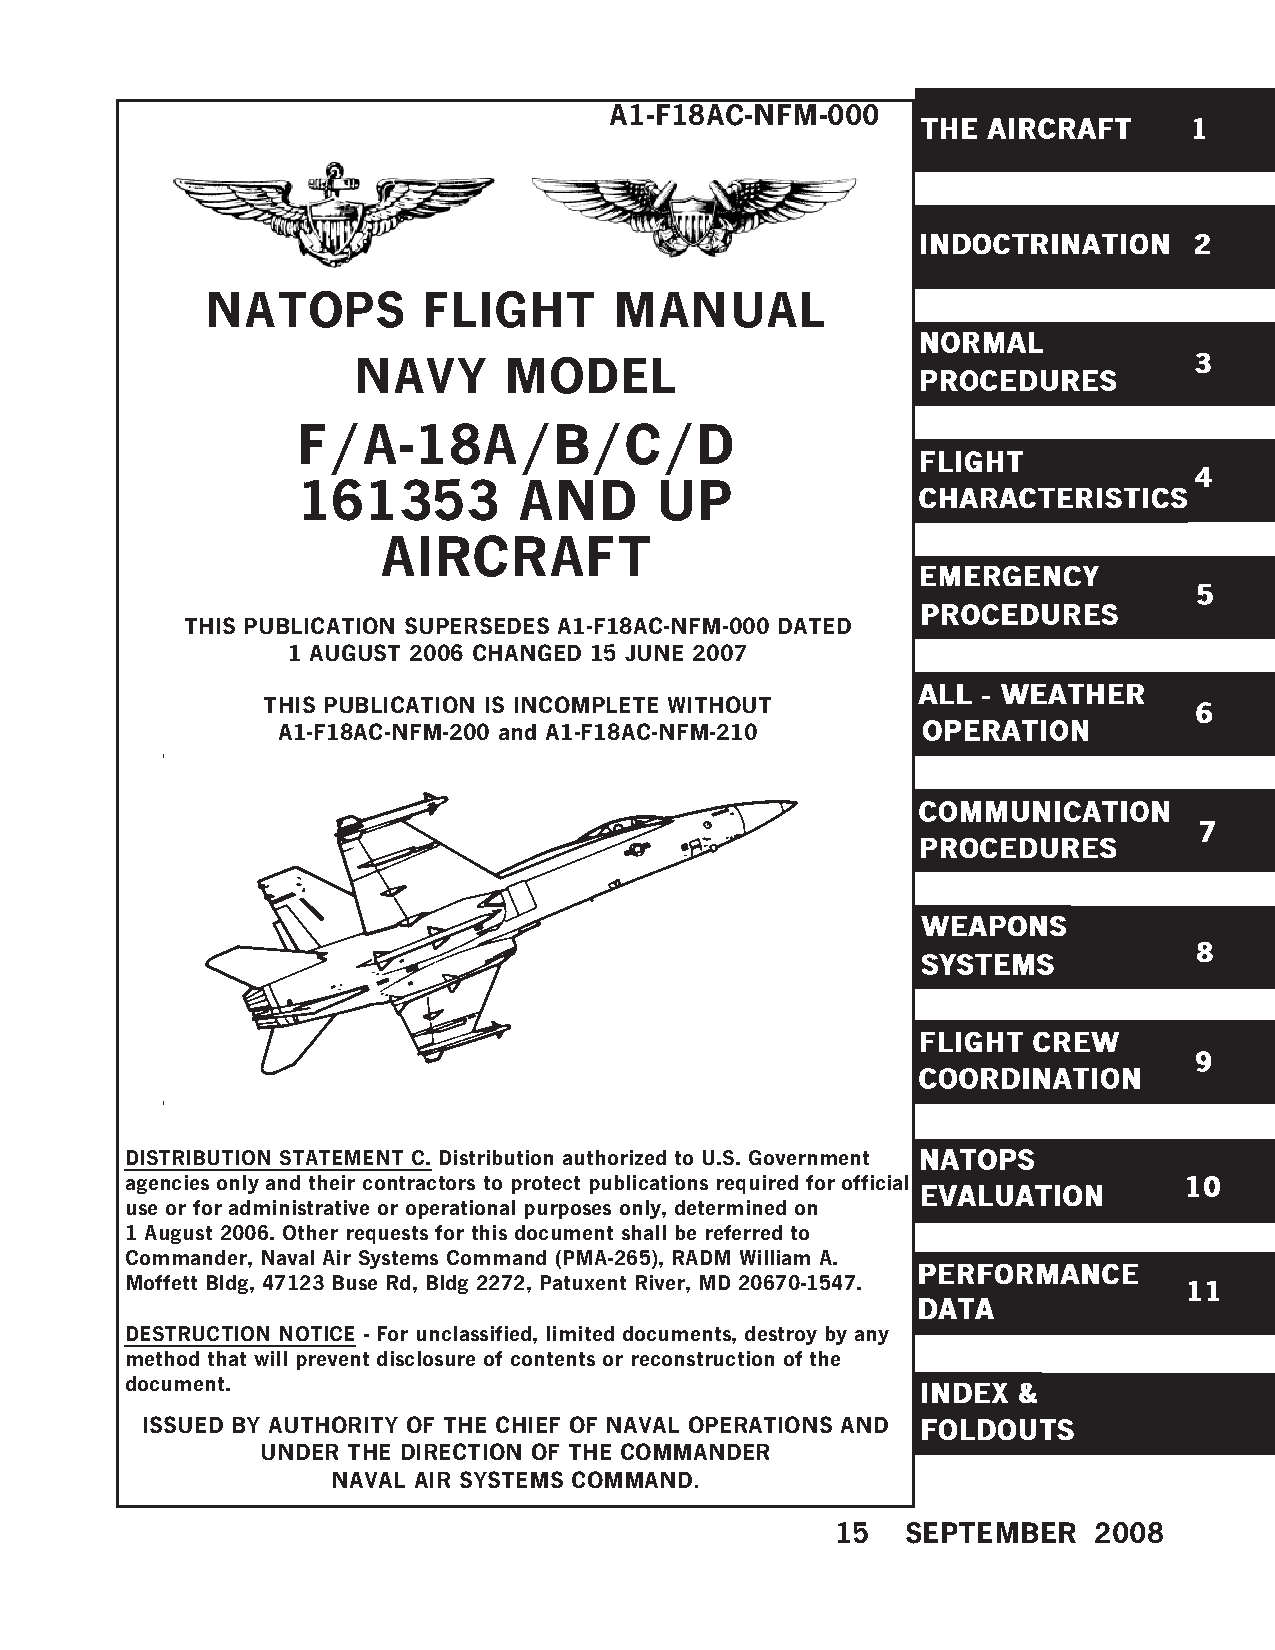
\includegraphics[
			width=0.8\linewidth,
			page = {1},
			trim = {3.0cm, 9.5cm, 8.0cm, 13cm},
			clip
		]{natops_F18C.pdf}
	};
	% Black area for white chevrons
	\fill[color1]
		([xshift=\outmar, yshift=0.2cm]current page text area.north east) --
		([xshift=\outmar, yshift=-\botmar]current page text area.south east) --
		([xshift=\chevin-0.5cm, yshift=-\botmar]current page text area.south east) --
		([xshift=\chevin-0.5cm, yshift=0.2cm]current page text area.north east) --
		cycle;
	\end{tikzpicture}
	% label for hyperrefs back to frontpage
	\label{frontpage}
	% make chevrons
	% use tabular for multi line node
	\thumbfront{Procedures}{0}
	\thumbfront{\begin{tabular}{c} Systems \end{tabular}}{1}
	\thumbfront{\begin{tabular}{c} APG-73 \\ Radar \end{tabular}}{2}
	\thumbfront{\begin{tabular}{c} TGP \\ JHMCS \end{tabular}}{3}
	\thumbfront{\begin{tabular}{c} A/G \\ Weapons \end{tabular}}{4}
	\thumbfront{\begin{tabular}{c} A/A \\ Weapons \end{tabular}}{5}
	\thumbwide

	\clearpage
	\null\vspace{0cm}

	\begin{tcolorbox}[
		enhanced, colback=white, colframe=color1, colbacktitle=white, coltitle=color1, sharp corners, attach boxed title to top center={yshift=2mm},
		boxed title style={
			sharp corners,
			drop shadow=color1!100
		}, title=\LARGE\textbf{DISCLAIMER}
	]
		\textbf{This document represents a personal project and is intended for entertainment purposes only. Do not use for training purposes or in real life scenarios.}
	\end{tcolorbox}

	\cleardoublepage

	\pagestyle{empty}
	\dominitoc
	\tableofcontents
	\cleardoublepage

	% restart page counter
	\setcounter{page}{1}
	% reactivate header and footer
	\pagestyle{body}

	\chapter{PROCEDURES}
	\thumbtab{Procedures}{0}
	\minitoc
	\cleardoublepage

	\section{START-UP}
	\subsection{PRE-START}
	\begin{tablenumerate}
		\blueitem{Ejection Seat test}{\textbf{DOWN \& ARMED}}
		\blueitem{Harness Lever}{\textbf{FWD}}
		\blueitem{Parking Brake}{\textbf{ENGAGED}}
		\blueitem{Master Arm}{\textbf{SAFE}}
	\end{tablenumerate}

	\subsection{ENGINE START}
	\begin{tablenumerate}
		\blueitem{Battery}{\textbf{ON}}
		\blueitem{Hyd. Brake}{> 3000psi}
		\blueitem{Fire Test}{
		\begin{subenumerate}
			\item \textbf{FIRE TEST} \dotfill \textbf{TEST A}
			\item \textbf{BATT} \dotfill cycle \textbf{OFF} then \textbf{ON}
			\item \textbf{FIRE TEST} \dotfill \textbf{TEST B}
		\end{subenumerate}}
		\blueitem{APU Start}{
		\begin{subenumerate}
			\item \textbf{APU Caution Light} \dotfill verify OFF
			\item \textbf{APU Switch} \dotfill \textbf{ON} \\
			\item \textbf{READY Light} \dotfill illuminated (30s)
		\end{subenumerate}}
		\blueitem{Right Engine Start}{
		\begin{subenumerate}
			\item \textbf{ENG CRANK} \dotfill \textbf{R}
			\item \textbf{R Eng RPM} \dotfill 15-25\%
			\item \textbf{R Throttle} \dotfill \textbf{IDLE}
		\end{subenumerate}}
		\blueitem{Stabilized Parameters}{
		\begin{subitemize}
			\item \textbf{IFEI} \dotfill Check
			\begin{itemize}
				\item \textbf{RPM} -- 60-65\%
				\item \textbf{EGT} -- < 750C until stable
			\end{itemize}
			\item \textbf{Cautions} \dotfill none for \textbf{ENG 2}
			\item \textbf{GPWS Voice Alerts} \dotfill Check
		\end{subitemize}}
		\blueitem{Master Caution}{\textbf{RESET}}
		\blueitem{Displays}{
		\begin{subenumerate}
			\item \textbf{Left DDI} \dotfill \textbf{ON}
			\item \textbf{Right DDI} \dotfill \textbf{ON}
			\item \textbf{AMPCD} \dotfill \textbf{ON}
		\end{subenumerate}}
		\blueitem{UFC}{
		\begin{subenumerate}
			\item \textbf{HUD} \dotfill \textbf{ON}
			\item \textbf{ALT Switch} \dotfill \textbf{RDR}
			\item \textbf{ATT Switch} \dotfill \textbf{AUTO}
		\end{subenumerate}}
		\blueitem{BLEED AIR Knob}{Cycle thru \textbf{OFF} to \textbf{NORM} \break (shutoff valves closed during fire test)}
		\blueitem{Left Engine Start}{
		\begin{subenumerate}
			\item \textbf{ENG CRANK} \dotfill \textbf{L}
			\item \textbf{L Eng RPM} \dotfill 15-25\%
			\item \textbf{L Throttle} \dotfill \textbf{IDLE}
		\end{subenumerate}}
		\blueitem{Stabilized Parameters}{
		\begin{subitemize}
			\item \textbf{IFEI} \dotfill Check
			\begin{itemize}
				\item \textbf{RPM} -- 60-65\%
				\item \textbf{EGT} -- < 750C until stable
			\end{itemize}
			\item \textbf{Cautions} \dotfill none for \textbf{ENG 1}
			\item \textbf{L GEN Caution} \dotfill Extinguished
		\end{subitemize}}
	\end{tablenumerate}

	\subsection{POST-START}
	\begin{tablenumerate}
		\blueitem{Canopy}{\textbf{CLOSED}}
		\blueitem{Start INS Align}{
		\begin{subenumerate}
			\item \textbf{INS Selector} \dotfill \textbf{GND} or \textbf{CV} (as required)
			\item \textbf{HSI} \dotfill select \textbf{STD HDG} (if available)\\
			\hfill \emph{(significantly reduces align time to approx. 90s)}
		\end{subenumerate}}
		\blueitem{RADAR}{\textbf{OPR}}
		\blueitem{FCS Reset}{
		\begin{subenumerate}
			\item \textbf{WING FOLD} \dotfill \textbf{SPREAD} \\
			\hfill \textbf{ONLY IF ON GROUND}
			\item \textbf{Left DDI} \dotfill \textbf{FCS} page
			\item \textbf{MASTER CAUTION} \dotfill \textbf{PRESS} twice \\ \hfill (restacks cautions)
			\item \textbf{FCS RESET} \dotfill \textbf{PRESS}
		\end{subenumerate}}
		\blueitem{Lights Test}{\textbf{Check}}
		\blueitem{Hook Bypass}{\textbf{As Required}}
		\blueitem{Flaps}{\textbf{HALF}}
		\blueitem{FCS BIT}{
		\begin{subenumerate}
			\item \textbf{BIT Failures} \dotfill press FCS-MC
			\item \textbf{MC1 \& MC2} \dotfill GO
			\item \textbf{FCSA \& FCSB} \dotfill PBIT GO
			\item \textbf{FCS BIT Switch} \dotfill press \& hold
			\item \textbf{FCS-MC} \dotfill press FCS OSB
			\item \textbf{FCSA \& FCSB} \dotfill GO
		\end{subenumerate}}
		\blueitem{ANTI SKID}{\textbf{OFF} if CV, else \textbf{ON}}
		\blueitem{Trim}{\textbf{PRESS T/O Trim}}
		\blueitem{PITOT}{\textbf{AUTO}}
		\blueitem{Displays}{
		\begin{subenumerate}
			\item \textbf{Left DDI} \dotfill \textbf{HUD Repeater}
			\item \textbf{Right DDI} \dotfill \textbf{FCS Page}
		\end{subenumerate}}
		\blueitem{RADALT Warning}{
		\begin{subitemize}
			\item \textbf{GND}\dotfill 200 ft
			\item \textbf{CV}\dotfill 80 ft
		\end{subitemize}}
		\blueitem{Standby Attitude Indicator}{\textbf{UNCAGED}}
		\blueitem{Bingo Fuel}{\textbf{As desired} (8000lbs)}
		\blueitem{Altimeter}{\textbf{Set}}
		\blueitem{Mission Data}{\textbf{ENTER}}
		\blueitem{Weapons/Sensors}{\textbf{As Required}}
		\blueitem{STORES Page}{\textbf{Verify proper inventory installed}}
		\blueitem{HMD Alignment}{
		\begin{subenumerate}
			\item \textbf{SUPT/HMD/ALIGN Page} \dotfill \textbf{SELECT}
			\item Superimpose \textbf{HMD} alignment cross on \textbf{HUD/BRU} alignment cross
			\item \textbf{CAGE/UNCAGE} \dotfill \textbf{PRESS \& HOLD} \\
			\hfill until \textbf{ALIGN OK}
		\end{subenumerate}

		\textbf{Fine Align}
		\begin{subenumerate}
			\item With \textbf{FA DXDY} displayed, use \textbf{TDC} to align azimuth and elevation \textbf{HMD} alignment crosses with \textbf{HUD/BRU} alignment cross
			\item \textbf{CAGE/UNCAGE} \dotfill \textbf{PRESS \& RELEASE}
			\item With \textbf{FA DROLL} displayed, use \textbf{TDC} to align roll axis \textbf{HMD} alignment crosses with \textbf{HUD/BRU} alignment cross
			\item \textbf{CAGE/UNCAGE} \dotfill \textbf{PRESS \& RELEASE}
		\end{subenumerate}}
		\blueitem{OBOGS}{\textbf{ON}}
		\blueitem{Complete INS Align}{\textbf{INS Selector} to \textbf{NAV} or \textbf{IFA} (if available)}
		\blueitem{Defensive Systems}{
		\begin{subenumerate}
			\item \textbf{ALR-67 RWR} \dotfill \textbf{ON}
			\item \textbf{ECM Selector} \dotfill \textbf{STBY}
			\item \textbf{Dispenser} \dotfill \textbf{ON} (middle)
		\end{subenumerate}}
		\blueitem{Lights}{
		\begin{subenumerate}
			\item \textbf{Strobe} \dotfill \textbf{ON}
			\item \textbf{POS Lights} \dotfill \textbf{BRT}
			\item \textbf{LDG/TAXI Lights} \dotfill \textbf{ON}
		\end{subenumerate}}
		\blueitem{Network}{
		\begin{subenumerate}
			\item \textbf{IFF} \dotfill \textbf{ON}
			\item \textbf{D/L} \dotfill \textbf{ON}, set desired frequency
		\end{subenumerate}}
		\blueitem{Parking Brake}{\textbf{DISENGAGE}}
		\blueitem{Chocks}{\textbf{REMOVED}}
		\blueitem{Audio}{\textbf{Volume as required}}
	\end{tablenumerate}

	\clearpage

	\section{TAKEOFF \& LANDING}

	\subsection{PRE-TAXI}
	\begin{tablenumerate}
		\blueitem{ANTI SKID}{As required
		\begin{subitemize}
			\item Field -- \textbf{ON}
			\item Carrier -- \textbf{OFF}
		\end{subitemize}}
		\blueitem{FLAPS}{\textbf{HALF}}
		\blueitem{CHOCKS}{\textbf{REMOVED}}
		\blueitem{LAUNCH BAR}{\textbf{RETRACTED}}
		\blueitem{HOOK BYPASS}{As required}
		\blueitem{PARKING BRAKE}{\textbf{DISENGAGED}}
	\end{tablenumerate}

	\subsection{TAKEOFF - SHORE}
	\begin{tablenumerate}
		\multicolumn{3}{c}{\textbf{After Lining Up On Runway}} \\
		\blueitem{ANTI SKID SPOILER BK}{\textbf{BOTH (UP)}}
		\blueitem{FLAPS}{\textbf{UP}}
		\blueitem{TRIM}{\textbf{T/O}}
		\blueitem{NWS}{\textbf{LOW GAIN}}
		\blueitem{Takeoff}{
		\begin{subenumerate}
			\item \textbf{BRAKES} \dotfill hold
			\item \textbf{THROTTLE} \dotfill \textbf{MIL}
			\item \textbf{BRAKES} \dotfill release
			\item \textbf{THROTTLE} \dotfill \textbf{MAX} \emph{if desired}
			\item \textbf{Rotation} \dotfill approx 150 KIAS \\
			\hfill \emph{hold 7 deg AOA}
			\item \textbf{GEAR} \dotfill \textbf{UP} < 240 KIAS
			\item \textbf{FLAPS} \dotfill \textbf{AUTO} once airborn
			\item \textbf{ALT} \dotfill \textbf{BARO} at 3000 agl
		\end{subenumerate}}
	\end{tablenumerate}

	\clearpage

	\subsection{TAKEOFF - CARRIER}
	\begin{tablenumerate}
		& \blue{Lineup} &
		\begin{subitemize}
			\item Wait behind JBD until Catapult is clear
			\item Follow Taxi Directors Instructions to line up on Catapult
		\end{subitemize} \\
		\blueitem{WING FOLD}{
		\begin{subenumerate}
			\item \textbf{WING FOLD} \dotfill \textbf{SPREAD} when directed \\
			\hfill wait until fully spread
			\item \textbf{WING FOLD} \dotfill \textbf{LOCK}
			\item \textbf{HUD Repeater} \dotfill no \textbf{WING UNLK} caution
		\end{subenumerate}}
		\blueitem{FLAPS}{\textbf{HALF}}
		\blueitem{Launch Bar Preparation}{
		\begin{subenumerate}
			\item \textbf{LAUNCH BAR} \dotfill \textbf{EXTEND} when directed
			\item \textbf{Throttle} \dotfill \textbf{UP} when directed
			\item \textbf{Taxi} \dotfill launch bar into shuttle
			\item \textbf{Throttle} \dotfill \textbf{IDLE} when directed
			\item \textbf{Wait} for holdback installation \& checks
			\item \textbf{LAUNCH BAR} \dotfill \textbf{RETRACT}
		\end{subenumerate}}
		\blueitem{Trim}{Refer to \textbf{NOTE} below}
		\blueitem{Speed Brakes}{\textbf{IN}}
		\blueitem{Final Checks}{
		\begin{subenumerate}
			\item \textbf{Throttle} \dotfill \textbf{MIL} when directed
			\item \textbf{Control Wipeout}
			\begin{itemize}
				\item Stick Full Forward
				\item Stick Full Aft
				\item Stick Full Left
				\item Stick Full Right
				\item Rudder Full Left
				\item Rudder Full Right
			\end{itemize}
			\item \textbf{Eng. Inst.} \dotfill \textbf{Checked}
			\item \textbf{Caution/Warnings}  \dotfill\textbf{None}
		\end{subenumerate}}
		\blueitem{Catapult Shot}{
		\begin{subenumerate}
			\item \textbf{Salute} \dotfill \textbf{CAT SHOT}
			\item \textbf{Gear} \dotfill \textbf{UP} < 240 KIAS
			\item \textbf{Flaps} \dotfill \textbf{AUTO}
			\item \textbf{ALT} \dotfill \textbf{BARO} at 3000 agl
		\end{subenumerate}}
		\blueitem{Clearing Turn}{}
	\end{tablenumerate}

	\notebox{
		\begin{itemize}
			\item Refer to \textbf{CHKLST} page for weight
		\end{itemize}
		\begin{center}
			\begin{tabular}{l | r | r | r}
				\toprule
				\textbf{Weight [lbs]} & $<$ 44000 & 44000-48000 & $>$ 48000 \\
				\midrule
				\textbf{Trim [deg]} & 16 & 17 & 18 \\
				\midrule
				\multicolumn{4}{c}{\textbf{MAX WEIGHT: 51900 lbs}} \\
				\bottomrule
			\end{tabular}
		\end{center}
	}

	\clearpage

	\subsection{LANDING - SHORE}
	\begin{center}
		\resizebox{0.95\linewidth}{!}{
			\includegraphics[
			page = {337},
			trim = {2cm, 2.8cm, 1.9cm, 2.7cm},
			clip
			]{natops_F18C.pdf}
		}
	\end{center}

	\clearpage

	\begin{tableitemize}
		\blueitem{Initial Approach}{
		\begin{subitemize}
			\item \textbf{HOOK} \dotfill \textbf{UP}
			\item \textbf{ANTI-SKID} \dotfill \textbf{ON}
			\item \textbf{ALT} \dotfill \textbf{RDR}\
			\item \textbf{Airspeed} \dotfill \textbf{300-350 KIAS}
			\item \textbf{Altitude} \dotfill \textbf{800 ft}
			\item \textbf{ARM} \dotfill \textbf{OFF}
		\end{subitemize}}
		\blueitem{Initial Break}{
		\begin{subitemize}
			\item \textbf{Break Interval} \dotfill \textbf{15-17 s}
			\item \textbf{SPEED BRAKE} \dotfill \textbf{EXTEND}
			\item \textbf{Throttle} \dotfill \textbf{IDLE}
			\item \textbf{G} \dotfill 1\% of Airspeed
			\item \textbf{Altitude} \dotfill \textbf{800 ft}
		\end{subitemize}}
		\blueitem{Break Turn}{
		\begin{subitemize}
			\item \textbf{Landing Gear} \dotfill \textbf{DOWN} at 250 KIAS
			\item \textbf{FLAPS} \dotfill \textbf{FULL} at 250 KIAS
			\item \textbf{SPEED BRAKE} \dotfill \textbf{RETRACT} at 250 KIAS
		\end{subitemize}}
		\blueitem{Downwind}{
		\begin{subitemize}
			\item \textbf{Altitude} \dotfill descend to \textbf{600 ft}
			\item \textbf{AOA} \dotfill \textbf{ON-SPEED}
			\item \textbf{LANDING CHECKLIST}
		\end{subitemize}}
		\blueitem{Final Turn}{
		\begin{subitemize}
			\item \textbf{Abeam Pos.} \dotfill \textbf{1-1.2 nmi}
		\end{subitemize}

		\textbf{90 Deg Position}
		\begin{subitemize}
			\item \textbf{AOA} \dotfill \textbf{ON-SPEED}
			\item \textbf{Altitude} \dotfill \textbf{400-500 ft}
		\end{subitemize}}
		\blueitem{Intercept Glideslope}{
		\begin{subitemize}
			\item \textbf{Distance} \dotfill \textbf{3/4 Mile}
			\item \textbf{Altitude} \dotfill \textbf{360 ft}
			\item \textbf{AOA} \dotfill \textbf{ON-SPEED}
		\end{subitemize}}
		\blueitem{Touchdown}{
		\begin{subitemize}
			\item No more than 750 ft/min
			\item \textbf{DO NOT FLARE}
		\end{subitemize}}
	\end{tableitemize}

	\subsection{LANDING - CARRIER CASE I}
	\begin{center}
		\resizebox{0.95\linewidth}{!}{
			\includegraphics[
			page = {356},
			trim = {1.9cm, 3.0cm, 2.0cm, 2.7cm},
			clip
			]{natops_F18C.pdf}
		}
	\end{center}

	\clearpage

	\begin{tablenumerate}
		\blueitem{Navigation}{
		\begin{subitemize}
			\item \textbf{TACAN} \dotfill \textbf{ON} and tuned
			\item \textbf{HSI}
			\begin{itemize}
				\item \textbf{TCN} -- \textbf{BOXED}
				\item \textbf{CRS} -- \textbf{BRC}
			\end{itemize}
		\end{subitemize}}
		\blueitem{Pattern Entry}{
		\begin{subitemize}
			\item \textbf{Distance} -- approx \textbf{5 nm}
			\item \textbf{Heading} -- \textbf{BRC}
			\item \textbf{Line Up} -- \textbf{Right of CV}
			\item \textbf{Airspeed} -- \textbf{300-350 KIAS}
			\item \textbf{Altitude} -- \textbf{800 ft}
		\end{subitemize}}
		\blueitem{Pre-Break}{
		\begin{subitemize}
			\item \textbf{HOOK} \dotfill \textbf{DOWN}
			\item \textbf{ALT} \dotfill \textbf{RDR}\
			\item \textbf{RADALT} \dotfill 370 ft
			\item \textbf{ANTI-SKID} \dotfill \textbf{OFF}
			\item \textbf{HOOK BYPASS} \dotfill \textbf{CARRIER}
			\item \textbf{ARM} \dotfill \textbf{OFF}
			\item \textbf{HSI Zoom} \dotfill 10 nm
			\item \textbf{Airspeed} \dotfill \textbf{300-350 KIAS}
			\item \textbf{Altitude} \dotfill \textbf{800 ft}
		\end{subitemize}}
		\blueitem{Initial Break}{
		\begin{subitemize}
			\item \textbf{Break Interval} \dotfill \textbf{15-17 s}
			\item \textbf{SPEED BRAKE} \dotfill \textbf{EXTEND}
			\item \textbf{Throttle} \dotfill \textbf{IDLE}
			\item \textbf{G} \dotfill 1\% of Airspeed
			\item \textbf{Altitude} \dotfill \textbf{800 ft}
		\end{subitemize}}
		\blueitem{Break Turn}{
		\begin{subitemize}
			\item \textbf{Landing Gear} \dotfill \textbf{DOWN} at 250 KIAS
			\item \textbf{FLAPS} \dotfill \textbf{FULL} at 250 KIAS
			\item \textbf{SPEED BRAKE} \dotfill \textbf{RETRACT} at 250 KIAS
		\end{subitemize}}
		\blueitem{Downwind}{
		\begin{subitemize}
			\item \textbf{Altitude} \dotfill descend to \textbf{600 ft}
			\item \textbf{AOA} \dotfill \textbf{ON-SPEED}
			\item \textbf{LANDING CHECKLIST}
		\end{subitemize}}
		\blueitem{Final Turn}{
		\begin{subitemize}
			\item \textbf{Abeam Pos.} \dotfill \textbf{1-1.2 nmi}
		\end{subitemize}

		\textbf{90 Deg Position}
		\begin{subitemize}
			\item \textbf{AOA} \dotfill \textbf{ON-SPEED}
			\item \textbf{Altitude} \dotfill \textbf{400-500 ft}
		\end{subitemize}}
		\blueitem{Intercept Glideslope}{
		\begin{subitemize}
			\item \textbf{Distance} \dotfill \textbf{3/4 Mile}
			\item \textbf{Altitude} \dotfill \textbf{360 ft}
			\item \textbf{AOA} \dotfill \textbf{ON-SPEED}
		\end{subitemize}}
		\blueitem{Touchdown}{
		\begin{subitemize}
			\item No more than 750 ft/min
			\item \textbf{DO NOT FLARE}
		\end{subitemize}}
	\end{tablenumerate}

	\notebox{
		\begin{itemize}
			\item \textbf{HSI} L wingtip will touch BRC line when 1.2nm abeam
			\item \textbf{HSI}  heading to boat is 5 deg behind abeam heading when rounddown visible
			\item \textbf{Tip} during approach turn, do not peak before the 90
		\end{itemize}
	}

	\vfill\null
	\clearpage


	\subsection{LANDING - CARRIER CASE III}
	\begin{center}
		\resizebox{0.95\linewidth}{!}{
			\includegraphics[
			page = {357},
			trim = {1.9cm, 2.9cm, 2.0cm, 2.7cm},
			clip
			]{natops_F18C.pdf}
		}
	\end{center}

	\begin{center}
		\large \textbf{Work In Progress} \normalsize
	\end{center}

	\subsection{LANDING - ICLS CASE III}
	\begin{center}
		\large \textbf{Work In Progress} \normalsize
	\end{center}

	\clearpage

	\section{IN-FLIGHT}

	\subsection{A/A REFUELING}
	\begin{center}
		\large \textbf{Work In Progress} \normalsize
	\end{center}

	\cleardoublepage

	\chapter{SYSTEMS}
	\thumbtab{Systems}{1}
	\minitoc
	\cleardoublepage

	\section{SYSTEMS}

	\subsection{ARC-210 RADIO}
	\begin{tableitemize}
		\blueitem{ARC-210}{
		\begin{subitemize}
			\item Provides T/R of AM/FM in 30-399.975MHz
			\item Contains 2 radios: COMM1 \& COMM2
			\item Controlled from UFC
		\end{subitemize}}
		\blueitem{Power On}{Rotate Vol knobs of COMM1 \& COMM2}
		\blueitem{Preset Channels}{
		\begin{subitemize}
			\item M: Manual
			\item 1-20: Preset Channels
			\item G: Guard (243.000)
			\item C: Cue Channel for SINCGARS
			\item S: Maritime (Sea)
		\end{subitemize}}
		\blueitem{OSB 1: GRCV}{Toggles Guard Receive}
		\blueitem{OSB 2: SQCH}{Toggles Squelch}
		\blueitem{OSB 3: CPHR}{Toggles Cipher modes (plain, cipher, delay) (not implemented)}
		\blueitem{OSB 4: AM / FM}{Selects Frequency Band}
		& & (only visible when in AM/FM overlap) \\
		\blueitem{OSB 5: MENU}{Menu Button}
		\blueitem{Manually Set Freq}{
		\begin{subenumerate}
			\item Set desired channel with channel knob
			\item Enter desired Frequency on UFC, ENT
			\item Confirm all options as desired
		\end{subenumerate}}
	\end{tableitemize}

	\subsection{AFCS - MODES}
	\begin{tableitemize}
		\blueitem{ATTH}{\textbf{Attitude Hold:} Aircraft will maintain existing pitch attitude and +/- 70 deg roll attitude}
		\blueitem{BALT}{\textbf{Barometric Altitude Hold:} Aircraft will maintain current heading and barometric altitude 0-70000 ft}
		\blueitem{HSEL}{\textbf{Heading Select:} Aircraft will turn and maintain heading selected on HSD}
		\blueitem{RALT}{\textbf{Radar Altitude Hold:} Aircraft will maintain current heading and radar altitude 0-5000 ft}
	\end{tableitemize}

	\subsection{AFCS - PROCEDURES}
	\begin{tableitemize}
		\blueitem{Conditions}{
		\begin{subitemize}
			\item Stick: Centered
			\item HSD: heading selected (if required)
		\end{subitemize}}
		\blueitem{Activation}{
		\begin{subenumerate}
			\item Press A/P OSB
			\item Select Submode OSB 
		\end{subenumerate}}
		\blueitem{Deactivation}{press Paddle Switch}
	\end{tableitemize}

	\subsection{ATC - APPROACH MODE}
	\begin{tableitemize}
		\blueitem{Conditions}{
		\begin{subitemize}
			\item Flaps: HALF/FULL
			\item TE Flaps: >27 deg
		\end{subitemize}}
		\blueitem{Activation}{ATC button}
		\blueitem{Effect}{Computer modulates thrust to maintain on speed AOA, pilot controls flightpath with pitch command}
		\blueitem{Deactivation}{ Any of the following:
		\begin{subitemize}
			\item ATC button
			\item Flaps: AUTO
			\item Weight On Wheels
			\item Bank Angle > 70deg
			\item Sensor Failure
		\end{subitemize}}
		\end{tableitemize}

	\subsection{ATC - CRUISE MODE}
	\begin{tableitemize}
		\blueitem{Conditions}{
		\begin{subitemize}
			\item Flaps: AUTO
		\end{subitemize}}
		\blueitem{Activation}{ATC button}
		\blueitem{Effect}{Computer modulates thrust to maintain existing airspeed}
		\blueitem{Deactivation}{
		\begin{subitemize}
			\item ATC button
			\item Flaps: HALF/FULL
			\item Sensor Failure
		\end{subitemize}}
	\end{tableitemize}

	\clearpage

	\section{NAVIGATION}

	\subsection{WAYPOINT}
	\begin{tableitemize}
		\blueitem{Waypoints}{Pre-planned navigational points of reference to follow on route to area of operation}
		& & Maximum: 60 \\
		\blueitem{Activate WAYPOINT Nav}{Press WYPT OSB on HSI}
		\blueitem{Select Sequence}{press SEQ\# OSB}
		\blueitem{Display Lines}{box SEQ on HSI}
		\blueitem{HSI Info (Top Right)}{Bearing (deg) / Distance (Nm)}
		& & Time-to-Go to Waypoint (min:sec) \\
		\blueitem{Automatic Sequencing}{box AUTO on HSI}
		& & Waypoint will automatically advance \\
	\end{tableitemize}

	\subsection{WAYPOINT - ADD}
	\begin{tablenumerate}
		\blueitem{DATA Page}{Press DATA OSB on HSI}
		& & verify correct sequence is selected \\
		\blueitem{Activate UFC}{press SEQUFC OSB}
		\blueitem{Insert Waypoint}{
		\begin{subenumerate}
			\item press INS OSB on UFC
			\item input desired number, ENT
		\end{subenumerate}}
		\blueitem{Edit Coordinates}{As described in \textbf{Section \ref{sec:wyptlatlong} or \ref{sec:wyptgrid}}}
	\end{tablenumerate}

	\subsection{WAYPOINT - REMOVE}
	\begin{tablenumerate}
		\blueitem{DATA Page}{Press DATA OSB on HSI}
		& & verify correct sequence is selected \\
		\blueitem{Activate UFC}{press SEQUFC OSB}
		\blueitem{Delete Waypoint}{
		\begin{subenumerate}
			\item press DEL OSB on UFC
			\item input desired number, ENT
		\end{subenumerate}}
	\end{tablenumerate}

	\subsection{WAYPOINT - EDIT LAT/LONG}
	\label{sec:wyptlatlong}
	\begin{tablenumerate}
		\blueitem{DATA Page}{Press DATA OSB on HSI}
		\blueitem{Select Waypoint}{using Increment/Decrement OSBs}
		\blueitem{Activate UFC}{
		\begin{subenumerate}
			\item press UFC OSB
			\item press POSN OSB
		\end{subenumerate}}
		\blueitem{Edit Coordinates}{
		\begin{subenumerate}
			\item Input Latitude, ENT
			\item Input Longitude, ENT
		\end{subenumerate}}
	\end{tablenumerate}

	\subsection{WAYPOINT - EDIT GRID COORDS}
	\label{sec:wyptgrid}
	\begin{tablenumerate}
		\blueitem{DATA Page}{Press DATA OSB on HSI}
		\blueitem{Select Waypoint}{using Increment/Decrement OSBs}
		\blueitem{Activate UFC}{
		\begin{subenumerate}
			\item press UFC OSB
			\item press GRID OSB
			\item HSI now displays Grid Menu
		\end{subenumerate}}
		\blueitem{Edit Coordinates}{
		\begin{subenumerate}
			\item Verify TDC slaved to HSI
			\item Press \& Hold TDC DEPRESS to slew
			\item Release TDC when over desired square
			\item Input remaining coords on UFC
		\end{subenumerate}}
	\end{tablenumerate}

	\subsection{WAYPOINT - PRECISE COORDS}
	\begin{tableitemize}
		\blueitem{Normal Coordinates}{
		\begin{subitemize}
			\item LAT/LONG: deg/min/sec
			\item GRID: 6 digits
		\end{subitemize}}
		\blueitem{Precise Coordinates}{
		\begin{subitemize}
			\item LAT/LONG: deg/min/sec.xx
			\item GRID: 10 digits
		\end{subitemize}}
		\blueitem{Activation}{
		\begin{subenumerate}
			\item press DATA OSB on HSI
			\item box PRECISE
		\end{subenumerate}}
	\end{tableitemize}

	\subsection{MARKPOINT}
	\begin{tableitemize}
		\blueitem{Markpoint}{Used to mark a point of interest}
		& & Maximum: 9 \\
		\blueitem{Activate Navigation}{
		\begin{subitemize}
			\item WYPT boxed on HSI
			\item M\# selected with Increment/Decrement OSBs
		\end{subitemize}}
		\blueitem{Examine MKPT Data}{press DATA OSB on HSI and select Markpoint as required}
		\blueitem{Employment}{
		\begin{subenumerate}
			\item Select desired markpoint with Increment / Decrement OSBs
			\item Box WPDSG OSB to designate markpoint as the target point
		\end{subenumerate}}
	\end{tableitemize}

	\subsection{MARKPOINT - ADD}
	\begin{tableitemize}
		\blueitem{Overfly Method}{
		\begin{subenumerate}
			\item Verify no target designated
			\item press MK\# OSB on HSI/SA to create Markpoint  on current location
		\end{subenumerate}}
		\blueitem{Target Designate \break Method}{
		\begin{subenumerate}
			\item Designate Target with sensor as required
			\item Press MK\# OSB on HSI/SA to create Markpoint on current designation
		\end{subenumerate}}
		\blueitem{Note}{After MK9 has been created the next Markpoint will overwrite MK1}
	\end{tableitemize}

	\subsection{ADF}
	\begin{tablenumerate}
		\blueitem{ADF Switch}{To desired COMM}
		\blueitem{Matching COMM}{Set ADF frequency as required (FM)}
		\blueitem{HSI}{Circle will appear indicating direction of ADF beacon on compass rose}
	\end{tablenumerate}

	\subsection{TACAN}
	\begin{tableitemize}
		\blueitem{TACAN}{Tactical Air Navigation}
		& & Provide direction \& distance to beacon \\
		\blueitem{UFC \break Activation}{
		\begin{subenumerate}
			\item Press TCN OSB and cycle to ON \\
			\item Verify T/R mode active
			\item Input channel \#\# , EN
			\item Set X/Y as required
			\item Set A/A mode if required
   		\end{subenumerate}}
		\blueitem{HSI \break Activation}{
			\begin{subenumerate}
				\item Box TCN OSB
				\item Set CRS as required
    		\end{subenumerate}}
		\blueitem{TACAN Data}{press DATA OSB on HSI while TCN boxed to view TACAN Database of all stations and their coordinates}
	\end{tableitemize}

	\cleardoublepage

	\subsection{AN/ALR-67 RWR}
	\begin{multicols*}{2}
		\begin{center}
			\begin{tabular}{c | p{1.5cm}  p{2.5cm}}
				\toprule
				\multicolumn{3}{c}{\blue{SURFACE}} \\
				\midrule
				\textbf{U} & & Unknown \\
				\textbf{S} & & Search Radar \\
				\textbf{T} & & ATC\\
				\midrule
				\textbf{3} & SA-3 & ``Goa" \\
				\textbf{6} & SA-6 & ``Gainful" \\
				\textbf{8} & SA-8 & ``Gecko" \\
				\midrule
				\textbf{10} & SA-10 & ``Grumble" \\
				\textbf{11} & SA-11 & ``Gadfly" \\
				\textbf{12} & SA-12 & ``Gladiator" \\
				\textbf{13} & SA-13 & ``Gopher" \\
				\midrule
				\textbf{40} & & Spruance Class \\
				\textbf{48} & & Nimitz Class \\
				\textbf{49} & & Perry Class \\
				\midrule
				\textbf{HK} & MIM-23 & Hawk \\
				\textbf{PT} & MIM-104 & Patriot \\
				\midrule
				\multicolumn{3}{c}{\blue{AIRBORNE}} \\
				\toprule
				\textbf{U} & & Unknown \\
				\textbf{M} & & Active missile \\
				\midrule
				\textbf{11} & F-111 &  Aardvark \\
				\textbf{13} & C-130 & Hercules \\
				\midrule
				\textbf{14} & F-14 & Tomcat \\
				\textbf{15} & F-15 & Eagle \\
				\textbf{16} & F-16 & Fighting Falcon \\
				\textbf{17} & C-17 & Globemaster III \\
				\textbf{18} & F/A-18 & Hornet \\
				\midrule
				\textbf{19} & MiG-19 & ``Farmer" \\
				\textbf{21} & MiG-21 & ``Fishbed" \\
				\textbf{22} & Tu-22 & ``Blinder" \\
				\textbf{23} & MiG-23 & ``Flogger" \\
				\textbf{24} & Su-24 & ``Fencer" \\
				\textbf{25} & MiG-25 & ``Foxbat" \\
				\midrule
				\textbf{29} & MiG-29 & ``Fulcrum" \\
				& Su-27 & ``Flanker" \\
				& Su-30 & ``Flanker-C" \\
				& Su-33 & ``Flanker-D" \\
				\midrule
			\end{tabular}
		\end{center}
		\columnbreak

		\begin{center}
			\begin{tabular}{c | p{1.5cm}  p{2.5cm}}
				\midrule
				\textbf{31} & MiG-31 & ``Foxhound" \\
				\textbf{34} & Su-34 & ``Fullback" \\
				\textbf{39} & Su-25M & ``Frogfoot" \\
				\midrule
				\textbf{52} & B-52 & Stratofortress \\
				\midrule
				\textbf{76} & IL-76 & ``Candid" \\
				\textbf{78} & IL-78 & ``Midas" \\
				\textbf{AN} & AN-26B & ``Curl" \\
				& AN-30M & ``Clank" \\
				\midrule
				\textbf{B1} & B-1 & Lancer \\
				\midrule
				\textbf{BE} & Tu-95 & ``Bear" \\
				\textbf{BF} & Tu-22 & ``Backfire" \\
				\textbf{BJ} & Tu-160 & ``Blackjack" \\
				\midrule
				\textbf{E2} & E-2 & Hawkeye \\
				\textbf{E3} & E-3 & Sentry \\
				\midrule
				\textbf{F4} & F-4 & Phantom \\
				\textbf{F-5} & F-5 & Tiger \\
				\midrule
				\textbf{HX} & Ka-27 & ``Helix" \\
				\midrule
				\textbf{KC} & KC-135 & Stratotanker \\
				\midrule
				\textbf{KJ} & KJ-2000 & ``Mainring" \\
				\textbf{M2} & Mirage 2k & \\
				\midrule
				\textbf{S3} & S-3 & Viking\\
				\textbf{SH} & SH-60 & Seahawk \\
				\bottomrule
			\end{tabular}
		\end{center}
	\end{multicols*}

	\subsection{AN/ALE-47 ACMDS}
	\begin{tableitemize}
		\blueitem{ACMDS}{Airborne Countermeasures Dispenser System}
		\blueitem{Conditions}{
		\begin{subitemize}
			\item Master Arm: ON
			\item DISPENSER Switch: ON (MIDDLE)
			\item ALE-47 Mode: not STBY
		\end{subitemize}}
		\blueitem{Self-Test}{Once airborne ALE-47 enters SF TEST before cycling to STBY}
		\blueitem{Set Mode}{MODE OSB with ALE-47 Boxed}
		\blueitem{Program Creation}{
		\begin{subenumerate}
			\item Box ALE-47 OSB
			\item Press ARM OSB
			\item Press CHAFF/FLAR OSBs, set \#
			\item press RPT OSB, set \# repetitions
			\item press INT OSB, set interval
			\item press SAVE OSB to save program
		\end{subenumerate}

		\begin{subitemize}
			\item \textbf{Note:} Use INCREMENT / DECREMENT OSBs to change values
		\end{subitemize}}
		\blueitem{Activation}{
		\begin{subitemize}
			\item Dispense Switch: AFT activates selected program
			\item Dispense Switch: FWD activates program 5 by default, can be cycled with STEP OSB
		\end{subitemize}}
	\end{tableitemize}

	\subsection{AN/ALE-47 ACMDS - MODES}
	\begin{tableitemize}
		\blueitem{MAN}{\textbf{Manual:} Program can be stored and edited, Chosen by pilot}
		\blueitem{AUTO}{\textbf{Automatic:} ALE-47 chooses when and what countermeasures to deploy}
		& & \textbf{Very Wasteful} \\
		\blueitem{S/A}{\textbf{Semi-Automatic:} ALE-47 chooses program. Pilot controls release}
		\blueitem{STBY}{\textbf{Standby Mode}}
	\end{tableitemize}

	\subsection{AN/ALQ-165 ASPJ}
	\begin{tableitemize}
		\blueitem{OFF}{Turns off ECM Pod}
		\blueitem{STBY}{Standby Mode}
		\blueitem{BIT}{ECM jammer pod Build-In-Test}
		\blueitem{REC}{\textbf{Receive Mode:} Jammer is passive
		\begin{subitemize}
			\item Collects information on detected radars
			\item Does NOT transmit jamming signal
		\end{subitemize}}
		\blueitem{X-MIT}{\textbf{Transmit Mode:} Jammer is active
		\begin{subitemize}
			\item ECM pod will automatically transmit jamming signal when radar lock detected on own aircraft
			\item When ASPJ is actively jamming own radar will be unavailable
		\end{subitemize}}
	\end{tableitemize}

	\subsection{DATALINK}
	\begin{center}
		\large \textbf{Work In Progress} \normalsize
	\end{center}

	\subsection{IFF}
	\begin{center}
		\large \textbf{Work In Progress} \normalsize
	\end{center}

	\subsection{SA PAGE}
	\begin{center}
		\large \textbf{Work In Progress} \normalsize
	\end{center}

	\cleardoublepage


	\chapter{AN/APG-73 RADAR}
	\thumbtab{AN/APG-73 Radar}{2}
	\minitoc
	\cleardoublepage

	\section{RWS - RANGE WHILE SEARCH}

	\subsection{RWS}
	\begin{tableitemize}
		\blueitem{Range While Scan}{\textbf{Default A/A Radar Mode}
		\begin{subitemize}
			\item Long range BVR mode. 
			\item Antenna follows designated search pattern and displays all tracks discovered in each sweep
		\end{subitemize}}
		\blueitem{Sensor Select Switch}{
		\begin{subitemize}
			\item \textbf{FWD:} Switch to ACM Boresight
			\item \textbf{AFT:} Assign TDC to AMPCD
			\item \textbf{LEFT:} Assign TDC to left DDI
			\item \textbf{RIGHT:} Assign TDC to right DDI
		\end{subitemize}}
	\end{tableitemize}

	\subsection{RWS - LTWS}
	\begin{tableitemize}
		\blueitem{Latent Track While Scan}{\textbf{RWS Submode}
		\begin{subitemize}
			\item Allows HAFU symbology for contacts and integration of offboard trackfiles
		\end{subitemize}}
		\blueitem{Activation}{DATA subpage on Radar Page}
		\blueitem{HAFU \break Symbology}{
		\begin{subitemize}
			\item Only displayed if TDC cursor is over trackfile or trackfile is L\&S or DT2
   			\item Offboard only tracks always displayed as HAFU
      		\item Launch acceptable ranges displayed for L\&S and DT2
		\end{subitemize}}
		\blueitem{IFF Interrogation}{Automatically when target under cursor}
	\end{tableitemize}

	\clearpage

	\section{TWS - TRACK WHILE SCAN}

	\subsection{TWS - DESIGNATION}
	\begin{tableitemize}
		\blueitem{Conditions}{
		\begin{subitemize}
			\item TWS selected 
			\item TDC slaved to current radar screen
		\end{subitemize}}
		\blueitem{L\&S \break (Primary Target)}{TDC DEPRESS while over trackfile}
		\blueitem{Cycle L\&S}{UNDESIGNATE Button (no DT2 designated)}
		\blueitem{DT2 (Secondary \break Target)}{TDC DEPRESS while over second trackfile}
		\blueitem{Swap L\&S DT2}{UNDESIGNATE Button}
		\blueitem{STT Lock}{TDC DEPRESS again over L\&S trackfile}
	\end{tableitemize}

	\subsection{TWS - SCAN CENTERING METHODS}
	\begin{tableitemize}
		\blueitem{MAN}{Manual: Azimuth centered on TDC cursor. Elevation can also be manually manipulated }
		\blueitem{AUTO}{Automatic: Azimuth, Elevation centered on L\&S trackfile. If L\&S trackfile lost returns to MAN }
		\blueitem{BIAS}{TDC DEPRESS on empty area to center azimuth there. Elevation controlled manually. Allows TDC to move separately from scan azimuth }
	\end{tableitemize}

	\subsection{TWS - SCAN RAID}
	\begin{tableitemize}
		\blueitem{SCAN RAID Mode}{
		\begin{subitemize}
			\item 22 deg, 3 bar scan centered on L\&S
			\item Radar will attempt to find multiple targets out of single target
		\end{subitemize}}
		\blueitem{Conditions}{
		\begin{subitemize}
			\item L\&S trackfile selected
		\end{subitemize}}
		\blueitem{Activation}{
		\begin{subitemize}
			\item RAID button
			\item RAID OSB
		\end{subitemize}}
		\blueitem{Deactivation}{
		\begin{subitemize}
			\item RAID deselect
			\item RSET OSB
			\item UNDESIGNATE button
			\item L\&S lost
		\end{subitemize}}
	\end{tableitemize}

	\subsection{TWS - EXP}
	\begin{tableitemize}
		\blueitem{EXP Mode}{10nm x 20 deg centered around L\&S}
		\blueitem{Conditions}{
		\begin{subitemize}
			\item L\&S trackfile selected
		\end{subitemize}}
		\blueitem{Activation}{EXP OSB}
		\blueitem{Deactivation}{
		\begin{subitemize}
			\item EXP OSB
			\item RSET OSB
			\item L\&S lost
		\end{subitemize}}
	\end{tableitemize}

	\clearpage

	\section{ACM - AIR COMBAT MANEUVERING}

	\subsection{ACM - BST}
	\begin{tableitemize}
		\blueitem{Boresight}{
		\begin{subitemize}
			\item $\pm$ 1.7 deg vertical
			\item $\pm$ 3.3 deg azimuth \\
			\item \textbf{Range:} 10nm \\
		\end{subitemize}}
		\blueitem{Conditions}{
		\begin{subitemize}
			\item Master Mode: A/A
			\item HMD: OFF
		\end{subitemize}}
		\blueitem{Activation}{SCS: FWD (enters BST)}
		\blueitem{Deactivation}{UNDESIGNATE button}
	\end{tableitemize}

	\subsection{ACM - VACQ}
	\begin{tableitemize}
		\blueitem{Vertical Acquis.}{
		\begin{subitemize}
			\item -13 deg to 46 deg vertical
			\item 6 deg azimuth \\
			\item Range: 5nm \\
		\end{subitemize}}
		\blueitem{Conditions}{
		\begin{subitemize}
			\item Master Mode: A/A
			\item HMD: OFF
		\end{subitemize}}
		\blueitem{Activation}{
		\begin{subenumerate}
			\item SCS: FWD (enters BST)
			\item then AFT (enters VACQ)
		\end{subenumerate}}
		\blueitem{Deactivation}{UNDESIGNATE button}
	\end{tableitemize}

	\subsection{ACM - WACQ}
	\begin{tableitemize}
		\blueitem{Caged Wide Acquis.}{
		\begin{subitemize}
			\item -9 deg to +6 deg vertical
			\item 60 deg azimuth
   		\end{subitemize}}
		\blueitem{Uncaged Wide Acquis.}{NOT IMPLEMENTED}
		\blueitem{Conditions}{
		\begin{subitemize}
			\item Master Mode: A/A
			\item HMD: OFF
		\end{subitemize}}
		\blueitem{Activation}{
		\begin{subenumerate}
			\item SCS: FWD (enters BST)
			\item then LEFT (enters WACQ)
		\end{subenumerate}}
		\blueitem{Toggle Mode}{CAGE/UNCAGE}
		\blueitem{Deactivation}{UNDESIGNATE button}
	\end{tableitemize}

	\subsection{ACM - GACQ}
	\begin{tableitemize}
		\blueitem{Gun Acquisition}{
		\begin{subitemize}
			\item -14 deg to +6 deg vertical
			\item 20 deg azimuth
		\end{subitemize}}
		\blueitem{Conditions}{
		\begin{subitemize}
			\item Master Mode: A/A
			\item HMD: OFF
		\end{subitemize}}
		\blueitem{Activation}{Automatically enabled upon guns selection}
		\blueitem{Deactivation}{UNDESIGNATE button}
	\end{tableitemize}

	\clearpage

	\section{LOCK ACQUISITION}

	\subsection{STT}
	\begin{tableitemize}
		\blueitem{Conditions}{
		\begin{subitemize}
			\item Master Mode: A/A
			\item TDC slaved to current radar scree
		\end{subitemize}}
		\blueitem{RWS Designation}{TDC DEPRESS to STT}
		\blueitem{LTWS Designation}{TDC DEPRESS to designate L\&S} & & second TDC DEPRESS to STT \\
		\blueitem{TWS Designation}{TDC DEPRESS to designate L\&S} & & second TDC DEPRESS to STT \\
		\blueitem{Undesignate}{UNDESIGNATE button}
	\end{tableitemize}

	\subsection{AACQ}
	\begin{tableitemize}
		\blueitem{Automatic Acquisition}{Fast method to acquire lock from BVR mode}
		\blueitem{Conditions}{
		\begin{subitemize}
			\item Master Mode: A/A
			\item TDC slaved to current radar screen
			\item Radar not in an ACM mode
		\end{subitemize}}
		\blueitem{Designation}{SCS towards radar screen}
		\blueitem{Deactivate}{SCS AFT}
	\end{tableitemize}

	\subsection{JHMCS}
	\begin{tableitemize}
		\blueitem{LHACQ}{Long Range Helmet Acquisition: 40nm}
		\blueitem{HACQ}{Helmet Acquisition: 10nm}
		\blueitem{Conditions}{
		\begin{subitemize}
			\item Master Mode: A/A
			\item HMD: BRT
		\end{subitemize}}
		\blueitem{LHACQ Activation}{SCS: FWD long (>0.8s)}
		\blueitem{HACQ Activation}{SCS: FWD short (<0.8s)}
		\blueitem{Deactivate}{SCS AFT}
	\end{tableitemize}

	\vfill\null
	\clearpage

	\section{MAP}

	\subsection{MAP}
	\begin{tableitemize}
		\blueitem{Conditions}{
		\begin{subitemize}
			\item Radar: OPR
		\end{subitemize}}
		\blueitem{Activation}{
		\begin{subitemize}
			\item Master Mode: A/G
			\item or SURF OSB on RDR ATTK page
		\end{subitemize}}
		\blueitem{PEN}{Scans small area on ground}
		\blueitem{FAN}{Broader/quicker scan, less defined image
		\begin{subitemize}
			\item narrow in azimuth, broad in elevation
   		\end{subitemize}}
	\end{tableitemize}

	\subsection{MAP - DESIGNATION}
	\begin{tableitemize}
		\blueitem{Conditions}{
		\begin{subitemize}
			\item Master Mode: A/G
			\item TDC slaved to current radar screen
		\end{subitemize}}
		\blueitem{Designation}{TDC DEPRESS while over desired location
		\begin{subitemize}
			\item Range will auto adjust \\
			\item Cross marks designated point on Radar \\
			\item Diamond marks designated point on HUD \\
		\end{subitemize}}
		\blueitem{Zoom}{using EXP1, EXP2, EXP3 modes}
		\blueitem{Undesignation}{UNDESIGNATE button}
	\end{tableitemize}

	\subsection{MAP - EXP1}
	\begin{tableitemize}
		\blueitem{EXP1}{
		\begin{subitemize}
			\item Lowest resolution expanded mode
			\item Range: 40nm
			\item Azimuth: 45deg
			\item Not ground stabilized unless designation exists (snowplow)
		\end{subitemize}}
		\blueitem{Conditions}{
		\begin{subitemize}
			\item Radar Mode: MAP
			\item TDC slaved to current radar screen
		\end{subitemize}}
		\blueitem{Activation}{
		\begin{subenumerate}
			\item EXP1 OSB
			\item Press \& hold TDC DEPRESS 
			\item Slew to desired region
			\item Release TDC DEPRESS
		\end{subenumerate}

		\begin{subitemize}
			\item Range will auto adjust
		\end{subitemize}}
		\blueitem{FAST Option}{Boxing FAST scan option doubles radar's rate of scan for approximately half the scan quality}
		\blueitem{Doppler Shift}{Area directly in front and at extreme edges of radar not visible}
		\blueitem{Deactivation}{UNDESIGNATE button}
	\end{tableitemize}

	\subsection{MAP - EXP2}
	\begin{tableitemize}
		\blueitem{EXP2}{
		\begin{subitemize}
			\item Next higher resolution from EXP1
			\item Range: 40nm
			\item Ground stabilized regardless if designation exists unless outside of radar gimbal limits
		\end{subitemize}}
		\blueitem{Conditions}{
		\begin{subitemize}
			\item Radar Mode: MAP
			\item or Radar Mode: EXP1
			\item TDC slaved to current radar screen
		\end{subitemize}}
		\blueitem{Activation}{
		\begin{subenumerate}
			\item EXP2 OSB
			\item Press \& hold TDC DEPRESS 
			\item Slew to desired region
			\item Release TDC DEPRESS
		\end{subenumerate}

		\begin{subitemize}
			\item Range will auto adjust
		\end{subitemize}}
		\blueitem{FAST Option}{Boxing FAST scan option doubles radar's rate of scan for approximately half the scan quality}
		\blueitem{Doppler Shift}{Area directly in front and at extreme edges of radar not visible}
		\blueitem{Deactivation}{UNDESIGNATE button}
	\end{tableitemize}

	\subsection{MAP - EXP3}
	\begin{tableitemize}
		\blueitem{EXP3}{
		\begin{subitemize}
			\item Synthetic-Aperture Radar (SAR) Map
			\item Range: 30nm
			\item Ground stabilized even w/o designation.
			\item 1.2 x 1.2nm, constant area and resolution regardless of range
		\end{subitemize}}
		\blueitem{Conditions}{
		\begin{subitemize}
			\item Radar Mode: MAP
			\item or Radar Mode: EXP1/EXP2
			\item TDC slaved to current radar screen
		\end{subitemize}}
		\blueitem{Activation}{
		\begin{subenumerate}
			\item EXP3 OSB
			\item Press \& hold TDC DEPRESS 
			\item Slew to desired region
			\item Release TDC DEPRESS
		\end{subenumerate}

		\begin{subitemize}
			\item Range will auto adjust
		\end{subitemize}}
		\blueitem{FAST Option}{Boxing FAST scan option doubles radar's rate of scan for approximately half the scan quality}
		\blueitem{Doppler Shift}{Area directly in front and at extreme edges of radar not visible}
		\blueitem{Deactivation}{UNDESIGNATE button}
	\end{tableitemize}

	\subsection{MAP - EXP DESIGNATION}
	\begin{tableitemize}
		\blueitem{Conditions}{
		\begin{subitemize}
			\item  Radar Mode: EXP (EXP3 recommended)
			\item TDC slaved to current radar screen
		\end{subitemize}}
		\blueitem{Activation}{
		\begin{subenumerate}
			\item Press \& hold TDC DEPRESS
			\item Slew to desired spot
			\item Release TDC DEPRESS to designate
		\end{subenumerate}}
		\blueitem{Symbology}{
		\begin{subitemize}
			\item Range will auto adjust
			\item Cross marks designated point on Radar
			\item Diamond marks designated point on HUD
		\end{subitemize}}
		\blueitem{TGP}{Targeting pod will automatically slave to designated point if FLIR ON and TGP unstowed}
		\blueitem{Deactivation}{UNDESIGNATE button}
	\end{tableitemize}

	\subsection{GMT}
	\begin{tableitemize}
		\blueitem{GMT Mode}{Ground Moving Target radar mode scans for highlights \& moving targets through doppler shift. Trackfiles displayed as bricks}
		\blueitem{Conditions}{
		\begin{subitemize}
			\item RDR: OPR
			\item Master Mode: A/G
		\end{subitemize}}
		\blueitem{Activation}{press MAP OSB from A/G MAP pag}
		\blueitem{Interleaved Option}{Press INTL OSB}
		& & GMT \& MAP modes interleaved, mode is GMT/MAP \\
	\end{tableitemize}

	\subsection{GMT - GMTT}
	\begin{tableitemize}
		\blueitem{GMTT}{Ground Moving Target Track}
		& & Range: 10nm \\
		\blueitem{Conditions}{
		\begin{subitemize}
			\item Master Mode: A/G
			\item TDC slaved to current radar screen
			\item Radar Mode: GMT
		\end{subitemize}}
		\blueitem{Activation}{1. \ Slew TDC over desired target}
		& & 2. \ SCS: Towards current radar screen to command acquisition \\
		\blueitem{Symbology}{
		\begin{subitemize}
			\item Radar page: brick with motion vector, speed, \& heading
			\item HUD: diamond
			\item point can be used/slaved to by other sensors
		\end{subitemize}}
		\blueitem{Deactivation}{UNDESIGNATE Button}
	\end{tableitemize}

	\subsection{SEA}
	\begin{tableitemize}
		\blueitem{SEA Mode}{SEA radar mode scans for highlights \& moving naval targets through doppler shift. Trackfiles displayed as bricks. Additional filtering applied \& scan rates reduced}
		\blueitem{Conditions}{
		\begin{subitemize}
			\item RDR: OPR
			\item Master Mode: A/G
		\end{subitemize}}
		\blueitem{Activation}{press MAP OSB from A/G MAP pag}
		\blueitem{Interleaved Option}{Press INTL OSB}
		& & GMT \& MAP modes interleaved, mode is SEA/MAP \\
	\end{tableitemize}

	\subsection{SEA - TARGET TRACKING}
	\begin{tableitemize}
		\blueitem{Conditions}{
		\begin{subitemize}
			\item Master Mode: A/G
			\item TDC slaved to current radar screen
			\item Radar Mode: SEA
		\end{subitemize}}
		\blueitem{Activation}{
		\begin{subenumerate}
				\item Slew TDC over desired target
				\item SCS: Towards current radar screen to command acquisition
		\end{subenumerate}}
		\blueitem{Symbology}{
		\begin{subitemize}
			\item Radar page: brick with motion vector, speed, \& heading
			\item HUD: diamond
			\item point can be used/slaved to by other sensors
		\end{subitemize}}
		\blueitem{Harpoon Conditions}{
		\begin{subitemize}
			\item Master Mode: A/G
			\item Target Locked
			\item HPD Mode: R/BL
		\end{subitemize}}
		\blueitem{Deactivation}{UNDESIGNATE Button}
	\end{tableitemize}

	\cleardoublepage

	\chapter{TGP \& JHMCS}
	\thumbtab{TGP \& JHMCS}{3}
	\minitoc
	\cleardoublepage

	\section{AAQ-28 LITENING II}

	\subsection{CONTROLS}
	\begin{tableitemize}
		\blueitem{Display Selection}{SCS: towards Targeting pod display}
		\blueitem{Toggle PTRK/ATRK}{SCS: towards Selected Display}
		\blueitem{Zoom}{
		\begin{subitemize}
			\item Radar Elevation Control
			\item Zoom OSBs
		\end{subitemize}}
		\blueitem{Toggle Wide/Nar FOV}{
		\begin{subitemize}
			\item RAID/FLIR Button short
			\item NAR/WIDE OSB
		\end{subitemize}}
		\blueitem{Toggle CCD/FLIR}{
		\begin{subitemize}
			\item RAID/FLIR Button long
			\item FLIR/CCD OS
		\end{subitemize}}
		\blueitem{Slew Reticle}{TDC Slew}
		\blueitem{Designate}{TDC DEPRESS}
		\blueitem{Undesignate}{NWS/UNDESIGNATE Button}
		\blueitem{Toggle LST}{CAGE/UNCAGE Button}
		\blueitem{Lase}{TRIGGER if TRIG mode boxed}
	\end{tableitemize}

	\subsection{POINTING METHODS}
	\begin{tableitemize}
		\blueitem{VVSLV}{FLIR slaved to line of sight of velocity vector}
		\blueitem{Snowplow}{Default mode when no Target designated}
		\blueitem{Stabilized Pointing}{Entered when target designated from Snowplow or cycled from ATRK/PTRK}
		\blueitem{Waypoint Slaving}{Available using HSI (TGP snaps to WYPT)}
		\blueitem{ATRK}{Tracks specific area. Best for fixed targets}
		\blueitem{PTRK}{Tracks specific Point. Best for moving targets}
	\end{tableitemize}

	\subsection{POINTING METHODS - VVSLV}
	\begin{tableitemize}
		\blueitem{VVSLV}{FLIR slaved to line of sight of velocity vector}
		\blueitem{Conditions}{
		\begin{subitemize}
			\item TDC slaved to current FLIR page
		\end{subitemize}}
		\blueitem{Activation}{
		\begin{subitemize}
			\item Press UNDESIGNATE twice
			\item or press VVSLV OSB on FLIR page
		\end{subitemize}}
		\blueitem{RTCL}{Box RTCL OSB to display TGP reticle}
		\blueitem{Designation}{TDC DEPRESS}
	\end{tableitemize}

	\subsection{POINTING METHODS - SNOWPLOW}
	\begin{tableitemize}
		\blueitem{Snowplow}{Default mode when no Target designated}
		& & \textbf{\textbullet} \ 0 deg left/right \\
		& & \textbf{\textbullet} \ -8 deg down \\
		\blueitem{Conditions}{
		\begin{subitemize}
			\item TDC slaved to current FLIR page
		\end{subitemize}}
		\blueitem{Activation}{1. \ Press UNDESIGNATE twice to select VVSLV \& unstow TGP}
		& & 2. \ Press UNDESIGNATE twice to deselect VVSLV \\
		\blueitem{Designation}{TDC DEPRESS}
	\end{tableitemize}

	\subsection{POINTING METHODS - STABILIZED POINTING}
	\begin{tableitemize}
		\blueitem{Stabilized Pointing}{FLIR can be slewed freely. Designated target is constantly updated to current location.}
		& & Ground stabilized \\
		\blueitem{Activation}{Entered automatically when}
		& & \textbf{\textbullet} \ Target designated from Snowplow \\
		& & \textbf{\textbullet} \ Cycled to from Auto Track or Point Track \\
		\blueitem{Designation}{Constantly updated}
	\end{tableitemize}

	\subsection{POINTING METHODS - WAYPOINT SLAVED}
	\begin{tableitemize}
		\blueitem{Conditions}{
		\begin{subitemize}
			\item TDC slaved to current FLIR page
			\item HSI: Desired waypoint selected
			\item HSI: WYPT boxed on
		\end{subitemize}}
		\blueitem{Activation}{HSI: press WPSDG to designate waypoint as target and slave TGP}
		\blueitem{Slew}{TDC slew to adjust TGP}
	\end{tableitemize}

	\subsection{POINTING METHODS - AREA TRACK}
	\begin{tableitemize}
		\blueitem{Conditions}{
		\begin{subitemize}
			\item TDC slaved to current FLIR page
		\end{subitemize}}
		\blueitem{Activation}{1. \ Unstow TGP with VVSLV}
		& & 2. SCS towards FLIR page to toggle ATRK/PTRK \\
		\blueitem{Slew}{Not possibe in Area Track}
		\blueitem{Designation}{TDC DEPRESS}
		\blueitem{Deactivation}{Press UNDESIGNATE to revert to Snowplow}
	\end{tableitemize}

	\subsection{POINTING METHODS - POINT TRACK}
	\begin{tableitemize}
		\blueitem{Conditions}{
		\begin{subitemize}
			\item TDC slaved to current FLIR page
		\end{subitemize}}
		\blueitem{Activation}{1. \ Unstow TGP with VVSLV}
		& & 2. SCS towards FLIR page to toggle ATRK/PTRK \\
		\blueitem{Slew}{Not possibe in Point Track}
		\blueitem{Designation}{TDC DEPRESS}
		\blueitem{Deactivation}{Press UNDESIGNATE to revert to Snowplow}
	\end{tableitemize}

	\subsection{POINTING METHODS - TGP OFFSET}
	\begin{tableitemize}
		\blueitem{Conditions}{
		\begin{subitemize}
			\item In ATRK/PTRK
		\end{subitemize}}
		\blueitem{OFFSET}{TDC DEPRESS to activate OFFSET}
		& & \textbf{\textbullet} \ + cross (Offset Cursor) appears \\
		& & \textbf{\textbullet} \ Slew with TDC \\
		\blueitem{Designation}{TDC DEPRESS again to designate Offset Cursor as new Target}
		\blueitem{FLIR to Cursor}{SCS in direction of FLIR page to snap TGP to location of Offset Cursor (while in PTRK)}
	\end{tableitemize}

	\subsection{START-UP \& LASING}
	\begin{tablenumerate}
		\blueitem{Start-Up}{
		\begin{subenumerate}
			\item FLIR Switch: STBY
			\item Open FLIR page, monitor warm-up
			\item FLIR Switch: ON when STBY displayed
			\item Confirm mode displays OPR
		\end{subenumerate}}
		\blueitem{Unstow}{
		\begin{subenumerate}
			\item Select VVSLV
			\item Unselect VVSLV to enter Snowplow
		\end{subenumerate}}
		\blueitem{DDI}{Contrast \& Brightness as required}
		\blueitem{LTD/R}{
		\begin{subenumerate}
			\item ARM
			\item Confirm L ARM indication
		\end{subenumerate}}
		\blueitem{TDC}{Slew to Target}
		\blueitem{Zoom}{as required (WIDE/NAR)}
		\blueitem{Camera Mode}{as required (CCD/FLIR)}
		\blueitem{Pointing Method}{as required}
		\blueitem{Laser Code}{
		\begin{subenumerate}
			\item Press UFC OSB
			\item Press LTDC, enter desired code
			\item Press ENT
		\end{subenumerate}}
		\blueitem{Designate Target}{TDC DEPRESS (will slave A/G weapons to TGP)}
		\blueitem{Lasing}{
		\begin{subitemize}
			\item TRIG boxed: press \& hold trigger to lase
			\item TRIG unboxed: AUTO lasing
	\end{subitemize}}
		\end{tablenumerate}

	\subsection{LASER SPOT TRACKER (LST)}
	\begin{tableitemize}
		\blueitem{Conditions}{
		\begin{subitemize}
			\item Master Mode: A/G
			\item TGP: ON
			\item LST/NFLR: ON
		\end{subitemize}}
		\blueitem{Set Laser Code}{1. \ UFC OSB on FLIR page}
		& & 2. \ Press LSTC, enter Code on Keypad, ENT \\
		\blueitem{Begin Search}{1. \ Set TGP to Snowplow, slew to vicinity of laser}
		& & 2. \ Press LST OSB on FLIR page, or press CAGE/UNCAGE \\
		\blueitem{Searching}{
		\begin{subitemize}
			\item FLIR image blank
			\item LST flashes on FLIR page
	\end{subitemize}}
		\end{tableitemize}

	\subsection{LASER MARKING}
	\blue{Note} CANNOT be used for weapons guidance, only visible in NVG
	\begin{checklistenumerate}
		\blueitem{TPOD}{\dotfill on and ready}
		\blueitem{LTD/R}{\dotfill ARM}
		\blueitem{SCS}{\dotfill press in direction of FLIR to focus}
		\blueitem{VVSLV}{\dotfill press UNDESIGNATE twice rapidly to select vel vector slave mode (or press VVSLV OSB)}
		\blueitem{Snowplow}{\dotfill press UNDESIGNATE twice rapidly to select snowplow mode(or press VVSLV OSB to deselect)}
		\blueitem{TDC}{\dotfill slew to target}
		\blueitem{TDC}{\dotfill depress to designate target}
		\blueitem{TRIG}{\dotfill boxed}
		\blueitem{MARK}{\dotfill boxed, activates M-Arm}
		\blueitem{Laser}{\dotfill press TRIGGER to mark \\ \hfill again to cease marking}
	\end{checklistenumerate}

	\subsection{A/A POINT TRACK}
	\begin{checklistenumerate}
		\blueitem{TPOD}{\dotfill on \& ready}
		\blueitem{Master Mode}{\dotfill A/A}
		\blueitem{SCS}{\dotfill in direction of FLIR display}
		\blueitem{VVSLV}{\dotfill press UNDESIGNATE twice rapidly to select vel vector slave mode (or press VVSLV OSB)}
		\blueitem{RTCL OSB}{\dotfill press to display reticle}
		\blueitem{Maneuver}{\dotfill to place vel. vector near target aircraft}
		\blueitem{Zoom}{\dotfill as desired}
		\blueitem{FLIR/CCD Mode}{\dotfill as desired}
		\blueitem{SCS}{\dotfill towards FLIR display to attempt Point Track}
		\blueitem{Designation Box}{\dotfill good track}
		\blueitem{Dump Target}{\dotfill SCS towards FLIR display}
	\end{checklistenumerate}
	To slave radar to TPOD
	\begin{checklistenumerate}
		\blueitem{Radar}{\dotfill OPR}
		\blueitem{Point Track}{\dotfill acquired}
		\blueitem{FLIR Page}{\dotfill press SLAVE OSB}
	\end{checklistenumerate}

	\subsection{A/A RADAR SLAVING}
	\begin{checklistenumerate}
		\blueitem{TPOD}{\dotfill on \& ready}
		\blueitem{Radar}{\dotfill OPR}
		\blueitem{Master Mode}{\dotfill A/A}
		\blueitem{R DDI}{\dotfill RDR ATTK page}
		\blueitem{L DDI}{\dotfill FLIR page}
		\blueitem{SCS}{\dotfill towards RDR ATTK page}
		\blueitem{Radar Lock}{\dotfill acquired}
		\blueitem{RRSLV OSB}{\dotfill press, slaves TPOD to radar}
		\blueitem{SCS}{\dotfill towards FLIR page}
		\blueitem{Zoom}{\dotfill as desired}
		\blueitem{FLIR/CCD Mode}{\dotfill as desired}
		\blueitem{SCS}{\dotfill towards FLIR page to attempt Point Track}
	\end{checklistenumerate}

	\cleardoublepage
	\section{ASQ-228 ATFLIR}

	\subsection{CONTROLS}
	\begin{tableitemize}
		\blueitem{Display Selection}{SCS: towards Targeting pod display}
		\blueitem{Toggle SCENE/AUTO}{SCS: towards Selected Display}
		\blueitem{Zoom}{
		\begin{subitemize}
			\item Radar Elevation Control
			\item Zoom OSBs
		\end{subitemize}}
		\blueitem{Toggle}{
		\begin{subitemize}
			\item RAID/FLIR Button short
		\end{subitemize}}
		\blue{WFOV/MFOV/NAR}& \textbf{\textbullet} \ FOV OSB \\
		\blueitem{Toggle CCD/FLIR}{
		\begin{subitemize}
			\item RAID/FLIR Button long
			\item FLIR/CCD OS
		\end{subitemize}}
		\blueitem{Slew Reticle}{TDC Slew}
		\blueitem{Designate}{TDC DEPRESS}
		\blueitem{Undesignate}{NWS/UNDESIGNATE Button}
		\blueitem{Lase}{TRIGGER if TRIG mode boxed}
	\end{tableitemize}

	\subsection{POINTING METHODS}
	\begin{tableitemize}
		\blueitem{VVSLV}{FLIR slaved to line of sight of velocity vector}
		\blueitem{Snowplow}{Default mode when no Target designated}
		\blueitem{Stabilized Pointing}{Entered when target designated from Snowplow or cycled from Auto Track / Point Track}
		\blueitem{Waypoint Slaving}{Available using HSI (TGP snaps to WYPT)}
		\blueitem{Scene Track}{Tracks specific area. Best for fixed targets}
		\blueitem{Auto Track}{Tracks specific Point. Best for moving targets}
		\blueitem{INR / Stabilized Pointing}{Active when TGP is slewed, maintains orientation to AC using inertial data}
	\end{tableitemize}

	\subsection{POINTING METHODS - VVSLV}
	\begin{tableitemize}
		\blueitem{VVSLV}{FLIR slaved to line of sight of velocity vector}
		\blueitem{Conditions}{
		\begin{subitemize}
			\item TDC slaved to current FLIR page
		\end{subitemize}}
		\blueitem{Activation}{
		\begin{subitemize}
			\item Press UNDESIGNATE twice
			\item or press VVSLV OSB on FLIR page
		\end{subitemize}}
		\blueitem{RTCL}{Box RTCL OSB to display TGP reticle}
		\blueitem{Designation}{TDC DEPRESS}
	\end{tableitemize}

	\subsection{POINTING METHODS - SNOWPLOW}
	\begin{tableitemize}
		\blueitem{Snowplow}{Default mode when no Target designated}
		& & \textbf{\textbullet} \ 0 deg left/right \\
		& & \textbf{\textbullet} \ -8 deg down \\
		\blueitem{Conditions}{
		\begin{subitemize}
			\item TDC slaved to current FLIR page
		\end{subitemize}}
		\blueitem{Activation}{1. \ Press UNDESIGNATE twice to select VVSLV \& unstow TGP}
		& & 2. \ Press UNDESIGNATE twice to deselect VVSLV \\
		\blueitem{Designation}{TDC DEPRESS}
	\end{tableitemize}

	\subsection{POINTING METHODS - WAYPOINT SLAVED}
	\begin{tableitemize}
		\blueitem{Conditions}{
		\begin{subitemize}
			\item TDC slaved to current FLIR page
			\item HSI: Desired waypoint selected
			\item HSI: WYPT boxed on
		\end{subitemize}}
		\blueitem{Activation}{HSI: press WPSDG to designate waypoint as target and slave TGP}
		\blueitem{Slew}{TDC slew to adjust TGP}
	\end{tableitemize}

	\subsection{POINTING METHODS - SCENE TRACK}
	\begin{tableitemize}
		\blueitem{Conditions}{
		\begin{subitemize}
			\item TDC slaved to current FLIR page
		\end{subitemize}}
		\blueitem{Activation}{1. \ Unstow TGP with VVSLV}
		& & 2. SCS towards FLIR page to toggle SCENE/AUTO \\
		\blueitem{Slew}{Scene Track reticle still slewable with TDC}
		\blueitem{Designation}{Automatic in SCENE Track}
		\blueitem{Deactivation}{Press UNDESIGNATE to revert to Snowplow}
	\end{tableitemize}

	\subsection{POINTING METHODS - AUTO TRACK}
	\begin{tableitemize}
		\blueitem{Conditions}{
		\begin{subitemize}
			\item TDC slaved to current FLIR page
		\end{subitemize}}
		\blueitem{Activation}{1. \ Unstow TGP with VVSLV}
		& & 2. SCS towards FLIR page to toggle SCENE/AUTO \\
		\blueitem{Slew}{Not possibe in Auto Track}
		\blueitem{Designation}{Automatic in AUTO Track}
		\blueitem{Deactivation}{Press UNDESIGNATE to revert to Snowplow}
	\end{tableitemize}

	\subsection{POINTING METHODS - TGP OFFSET}
	\begin{tableitemize}
		\blueitem{Conditions}{
		\begin{subitemize}
			\item AUTO Track
		\end{subitemize}}
		\blueitem{OFFSET}{TDC DEPRESS to activate OFFSET}
		& & \textbf{\textbullet} \ + cross (Offset Cursor) appears \\
		& & \textbf{\textbullet} \ Slew with TDC \\
		\blueitem{Designation}{SCS towards FLIR to designate Offset Cursor}
		\blueitem{FLIR to Cursor}{SCS in direction of FLIR page to snap TGP to location of Offset Cursor (while in PTRK)}
	\end{tableitemize}

	\subsection{LASER SPOT TRACKER (LST)}
	\begin{tableitemize}
		\blueitem{Conditions}{
		\begin{subitemize}
			\item Master Mode: A/G
			\item TGP: ON
			\item LST/NFLR: ON
		\end{subitemize}}
		\blueitem{Set Laser Code}{1. \ UFC OSB on FLIR page}
		& & 2. \ Press LSTC, enter Code on Keypad, ENT \\
		\blueitem{Begin Search}{1. \ Set TGP to Snowplow, slew to vicinity of laser}
		& & 2. \ Press LST OSB on FLIR page \\
		\blueitem{Searching}{
		\begin{subitemize}
			\item FLIR image blank
			\item LST flashes on FLIR page
		\end{subitemize}}
		\blueitem{Designation}{TDC DEPRESS}
	\end{tableitemize}

	\subsection{A/A OPERATION MODES}
	\subsection{A/A AUTO TRACK}
	\subsection{A/A L+S SLAVE}

	\cleardoublepage
	\section{JHMCS}

	\subsection{CONTROLS}
	\begin{tableitemize}
		\blueitem{HMD Brightness}{BRT}
		& & Powers on JHMCS \\
		\blueitem{Master Mode}{A/A \& A/G Master Mode buttons}
		& & symbology changes depending on selected mode \\
		\blueitem{HMD Blanking Toggle}{Even Marker ``Recce" Button}
		& & Toggles manual blanking \\
		\blueitem{LHACQ Activation}{
		\begin{subitemize}
			\item Master Mode: A/A
			\item SCS: FWD long (>0.8s)
		\end{subitemize}}
		\blueitem{HACQ Activation}{
		\begin{subitemize}
			\item Master Mode: A/A
			\item SCS: FWD short  (<0.8s)
		\end{subitemize}}
		\blueitem{Toggle Selected Sensor}{
		\begin{subitemize}
			\item Master Mode: A/G
			\item SCS: FWD
			\item Toggles between HUD and HMD \\
		\end{subitemize}}
		\blueitem{Undesignate}{UNDESIGNATE}
	\end{tableitemize}

	\subsection{SYMBOLOGY}

	\subsection{SETUP - FORMAT}

	\subsection{SETUP - BLANKING}

	\subsection{SETUP - REJECT}

	\subsection{SETUP - MIDS}

	\subsection{TARGET DESIGNATION - A/G}
	\begin{tableitemize}
		\blueitem{Conditions}{
		\begin{subitemize}
			\item Master Mode: A/G
			\item JHMCS: ON
			\item TDC slaved to HUD or HMD
		\end{subitemize}}
		\blueitem{Symbology}{
		\begin{subitemize}
			\item HUD: dot in VV indicates HUD slaved
			\item HMD: Aiming Reticle indicates HMD slaved
		\end{subitemize}}
		\blueitem{Designation}{TDC DEPRESS}
		\blueitem{Slew Diamond}{TDC slew}
		\blueitem{Undesignate}{UNDESIGNATE}
	\end{tableitemize}

	\subsection{TARGET DESIGNATION - A/A Radar}
	\begin{tableitemize}
		\blueitem{LHACQ}{Long Range Helmet Acquisition: 40nm}
		\blueitem{HACQ}{Helmet Acquisition: 10nm}
		\blueitem{Conditions}{
		\begin{subitemize}
			\item Master Mode: A/A
			\item HMD: BRT
		\end{subitemize}}
		\blueitem{LHACQ Activation}{SCS: FWD long (>0.8s)}
		\blueitem{HACQ Activation}{SCS: FWD short (<0.8s)}
		\blueitem{Deactivate}{SCS AFT}
	\end{tableitemize}

	\subsection{AIM-9X - UP-LOOK}
	\begin{tableitemize}
		\blueitem{Up-Look}{Slaves AIM-9X to Up-Look reticle}
		& & (significantly above HMD Line of Sight) \\
		\blueitem{Conditions}{
		\begin{subitemize}
			\item Master Mode: A/A
			\item HMD: BRT
			\item AIM-9X: Selected
		\end{subitemize}}
		\blueitem{Activation}{SCS: FWD (slave TDC to HMD)}
		\blueitem{Uncage}{CAGE/UNCAGE button}
	\end{tableitemize}

	\cleardoublepage
	\chapter{A/G WEAPONS}
	\thumbtab{A/G}{4}
	\minitoc
	\cleardoublepage

	\section{A/G OVERVIEW}
	\begin{center}
		\begin{tabular}{l | c | p{6cm}}
			\toprule
			\blue{Weapon} & \blue{SMS} & \blue{Type}\\
			\midrule
			\multicolumn{3}{c}{\blue{Unguided}} \\
			\midrule
			\textbf{LAU-61} & 61S/R &  2.75-in Hydra rockets (19x) \\
			\textbf{LAU-68} & 68S/R &  2.75-in Hydra rockets (7x) \\
			\textbf{LAU-10} & 10S/R &  5-in Zuni rockets (4x) \\
			\midrule
			\textbf{MK-82} & 82B & 500 lbs  low-drag unguided bomb \\
			\textbf{MK-82 SE} & 82XT & 500 lbs  retarded unguided bomb \\
			\textbf{MK-82 Bal} & 82YT & 500 lbs  retarded unguided bomb \\
			\textbf{MK-83} & 83B & 1000 lbs  low-drag unguided bomb \\
			\textbf{MK-84} & 84 & 2000lbs  low-drag unguided bomb \\
			\midrule
			\textbf{BDU-33} & & 25 lbs  unguided training bomb \\
			\midrule
			\textbf{MK-20 RE} & RE & 500 lbs Unguided cluster bomb \\
			\textbf{CBU-99} & RET & 500 lbs anti-tank cluster bomb \\
			\midrule
			\multicolumn{3}{c}{\blue{Laser-Guided Bombs}} \\
			\midrule
			\textbf{GBU-12} & 82LG & 500 lbs PAVEWAY II LGB \\
			\textbf{GBU-16} & 83LG & 1000 lbs PAVEWAY II LGB \\
			\textbf{GBU-10} & 84LG & 2000 lbs PAVEWAY II LGB \\
			\textbf{GBU-24} & GB24 & 2000 lbs PAVEWAY III LGB Penetrator \\
			\midrule
			\multicolumn{3}{c}{\blue{GPS Munitions}} \\
			\midrule
			\textbf{GBU-38} & J-82 & 500 lbs JDAM \\
			\textbf{GBU-32} & J-83 & 1000 lbs JDAM \\
			\textbf{GBU-31} & J-84 & 2000 lbs JDAM \\
			\textbf{GBU-31(V)} & J-109 & 2000 lbs JDAM Penetrator \\
			\midrule
			\textbf{AGM-154A} & JSA & JSOW Cluster \\
			\textbf{AGM-154C} & JSC & JSOW Penetrator \\
			\midrule
			\multicolumn{3}{c}{\blue{A/G Missiles}} \\
			\midrule
			\textbf{AGM-65E} & MAV & Laser Guided A/G missile\\
			\textbf{AGM-65F} & MAVF & IR Guided A/G missile\\
			\midrule
			\textbf{AGM-88C} & HARM & High-Speed Anti-Radiation Missile\\
			\midrule
			\textbf{AGM-84D} & HPD & Harpoon anti-ship missile \\
			\textbf{AGM-84E} & SLMR & SLAM-ER \\
			\midrule
			\textbf{AGM-62} & WEDL & 2000 lbs TV-guided bomb \\
			\bottomrule
		\end{tabular}
	\end{center}

	\clearpage

	\section{SELECTIVE ORDNANCE JETTISON}
	\begin{checklistenumerate}
		\blueitem{Master Arm}{\dotfill ARM}
		\blueitem{SMS}{\dotfill check stores}
		\blueitem{Jettison Stores}{\dotfill select desired \\ \hfill jettison stations on pushbuttons}
		\blueitem{Selective Jett. Knob}{\dotfill rotate to \\ \hfill desired stations}
		\blueitem{Jett. Button}{\dotfill press \& hold}
		\blueitem{Selective Jett. Knob}{\dotfill SAFE}
	\end{checklistenumerate}

	\section{FORWARD FIRING}

	\subsection{M61A2 GUN - A/G}
	\begin{checklistenumerate}
		\blueitem{Master Arm}{\dotfill ARM}
		\blueitem{Master Mode}{\dotfill A/G}
		\blueitem{SMS}{\dotfill select GUN
		\begin{subitemize}
			\item \blue{Rounds} MK-50 or PGU-28
			\item \blue{Firing Rate} HI or LO
			\item \blue{Mode} CCIP
		\end{subitemize}}
		\blueitem{Reticle}{\dotfill on target}
		\blueitem{Fire}{\dotfill once IN RNG cue}
		\blueitem{Break Away}{\dotfill before X cue}
	\end{checklistenumerate}

	\subsection{ROCKETS}
	\begin{checklistenumerate}
		\blueitem{Master Arm}{\dotfill ARM}
		\blueitem{Master Mode}{\dotfill A/G}
		\blueitem{SMS}{\dotfill select pod (68R)
		\begin{subitemize}
			\item \blue{Firing Mode} SGL or SAL
			\item \blue{MTR} M4 or M66
			\item \blue{Mode} CCIP
		\end{subitemize}}
		\blueitem{Reticle}{\dotfill on target}
		\blueitem{Fire}{\dotfill once IN RNG cue appears}
		\blueitem{Break Away}{\dotfill before X cue}
	\end{checklistenumerate}

	\clearpage

	\section{UNGUIDED FREE-FALL MUNITIONS}

	\subsection{UNGUIDED BOMB - CCIP}
	\begin{checklistenumerate}
		\blueitem{Master Arm}{\dotfill ARM}
		\blueitem{Master Mode}{\dotfill A/G}
		\blueitem{SMS}{\dotfill select desired bomb (82B)
		\begin{subenumerate}
			\item Create delivery PROG 1
			\item \blue{Mode}\dotfill CCIP
			\item \blue{MFUZ}\dotfill NOSE
			\item \blue{EFUZ}\dotfill DLY1 or INST
			\item \blue{DRAG}\dotfill FF or RET based on bomb type
		\end{subenumerate}}
		\blueitem{UFC}{\dotfill press UFC OSB on SMS page
		\begin{subitemize}
			\item \blue{QTY} bombs per release
			\item \blue{MULT} bombs per salvo in release
			\item \blue{INT} interval between salvo in feet
		\end{subitemize}}
		\blueitem{Dive}{\dotfill 30-45 deg}
		\blueitem{DIL}{\dotfill Displayed Impact Line over target}
		\blueitem{CCIP Cross}{\dotfill appears once computed}
		\blueitem{Maneuver}{\dotfill keep CCIP CROSS \& DIL on target}
		\blueitem{Release}{\dotfill when CCIP CROSS on target}
		\blueitem{Pull Up}{\dotfill before vel vector reaches PULL UP cue}
	\end{checklistenumerate}

	\subsection{UNGUIDED BOMB - CCRP}
	\begin{checklistenumerate}
		\blueitem{Master Arm}{\dotfill ARM}
		\blueitem{Master Mode}{\dotfill A/G}
		\blueitem{SMS}{\dotfill select desired bomb (82B)
		\begin{subenumerate}
			\item Create delivery PROG 1
			\item \blue{Mode}\dotfill CCRP
			\item \blue{MFUZ}\dotfill NOSE
			\item \blue{EFUZ}\dotfill DLY1 or INST
			\item \blue{DRAG}\dotfill FF or RET based on bomb type
		\end{subenumerate}}
		\blueitem{UFC}{\dotfill press OSB for UFC on SMS page
		\begin{subitemize}
			\item \blue{QTY} bombs per release
			\item \blue{MULT} bombs per salvo in release
			\item \blue{INT} interval between salvo in feet
		\end{subitemize}}
		\blueitem{SCS}{\dotfill FWD to slave TDC to HUD}
		\blueitem{Symbology}{\dotfill ``Ball \& Chain"}
		\blueitem{Dive}{\dotfill 25 deg to place vel vector on target}
		\blueitem{TDC}{\dotfill DEPRESS to designate target}
		\blueitem{TDC}{\dotfill SLEW target designator}
		\blueitem{Level Flight}{\dotfill keep vel vector aligned with ASL (azimuth steering line)}
		\blueitem{Release}{\dotfill when weapon cue appears, hold until all ordnance released}
		\blueitem{Pull Up}{\dotfill before vel vector reaches PULL UP cue}
	\end{checklistenumerate}

	\subsection{MK-20 CLUSTER BOMB - CCIP}
	\begin{checklistenumerate}
		\blueitem{Master Arm}{\dotfill ARM}
		\blueitem{Master Mode}{\dotfill A/G}
		\blueitem{SMS}{\dotfill select desired bomb (RE)
		\begin{subenumerate}
			\item Create delivery PROG 1
			\item \blue{Mode}\dotfill CCIP
			\item \blue{MFUZ}\dotfill VT
			\item \blue{HT OSB}\dotfill press to cycle
		\end{subenumerate}}
		\blueitem{UFC}{\dotfill press UFC OSB on SMS page
		\begin{subitemize}
			\item \blue{QTY} bombs per release
			\item \blue{MULT} bombs per salvo in release
			\item \blue{INT} interval between salvo in feet
		\end{subitemize}}
		\blueitem{Dive}{\dotfill 30-45 deg}
		\blueitem{DIL}{\dotfill Displayed Impact Line over target}
		\blueitem{CCIP Cross}{\dotfill appears once computed}
		\blueitem{Maneuver}{\dotfill keep CCIP CROSS \& DIL on target}
		\blueitem{Release}{\dotfill when CCIP CROSS on target}
		\blueitem{Pull Up}{\dotfill before vel vector reaches PULL UP cue}
	\end{checklistenumerate}

	\clearpage

	\section{GPS GUIDED MUNITIONS}

	\subsection{JDAM/JSOW - PP}
	\blue{Weapon Setup}
	\begin{checklistenumerate}
		\blueitem{Coord.}{\dotfill prepare in format \\ \hfill DEG MIN SEC : DEC-SEC}
		\blueitem{SMS}{\dotfill while on ground
		\begin{subenumerate}
			\item Select desired JDAM (J-82) or JSOW (JSA/JSC)
			\item \blue{Wait}\dotfill for GOOD align (3 min)
			\item \blue{Mode}\dotfill PP
			\item \blue{Fuzing}\dotfill INST
		\end{subenumerate}}
		\blueitem{JDAM Display}{\dotfill press JDAM DSPLY OSB}
		\blueitem{Release Type}{\dotfill MANUAL}
		\blueitem{QTY}{\dotfill press QTY OSB select desired stations (recommend: all) press RTN OSB, now STEP OSB cycles between stations}
		\blueitem{MSN Page}{\dotfill crossed out PP mean no coordinates}
		\blueitem{Select PP1}{\dotfill press PP1 OSB}
		\blueitem{Data Entry}{\dotfill press TGT UFC OSB
		\begin{subenumerate}
			\item \blue{HT}\dotfill enter height for cluster\\
			\hfill dispersal (only for JSA)
			\item \blue{Return}\dotfill press TGT UFC twice\\
			\hfill to return to main UFC page
			\item \blue{ELEV}\dotfill select ELEV on UFC
			\item \blue{Return}\dotfill press TGT UFC twice\\
			\hfill to return to main UFC page
			\item \blue{POSN}\dotfill select POSN on UFC
			\item \blue{LAT}\dotfill input DEG MIN SEC, ENT \\
			\hfill  input DEC-SEC, ENT
			\item \blue{LON}\dotfill input DEG MIN SEC, ENT \\
			\hfill input DEC-SEC, ENT
			\item \blue{Return}\dotfill press TGT UFC twice\\
			\hfill  to return to main UFC page
		\end{subenumerate}}
		\blueitem{Verify}{\dotfill PP1 no longer crossed}
		\blueitem{Repeat}{\dotfill for remaining stations}
  	\end{checklistenumerate}
	

	\blue{Weapon Launch}
	\begin{checklistenumerate}
		\blueitem{Master Arm}{\dotfill ARM}
		\blueitem{Master Mode}{\dotfill A/G}
		\blueitem{SMS}{\dotfill verify J-82 boxed}
		\blueitem{R DDI}{\dotfill HSI page}
		\blueitem{L DDI}{\dotfill JDAM page}
		\blueitem{Verify}{\dotfill MANUAL release, PP, desired station}
		\blueitem{Maneuver}{\dotfill with steering cues}
		\blueitem{TMR}{\dotfill Time to Minimum Range}
		\blueitem{IN RNG}{\dotfill In Range}
		\blueitem{Fire}{\dotfill hold weapon release}
		\blueitem{Next}{\dotfill system will auto cycle to next JDAM}
		\blueitem{Verify}{\dotfill MANUAL release, PP, desired station}
		\blueitem{Repeat}{\dotfill for remaining bombs}
	\end{checklistenumerate}

	\blue{Note} each JDAM can have 4 PP targets

	\subsection{JDAM/JSOW - TOO WYPT}
	\blue{Weapon Setup}
	\begin{checklistenumerate}
		\blueitem{Waypoints}{\dotfill verify
		\begin{subenumerate}
			\item \blue{SUPT HSI}
			\item \blue{DATA}\dotfill cycle through waypoints
			\item \blue{Precise}\dotfill push PRECISE OSB to add DEC-SEC
		\end{subenumerate}}
		\blueitem{SMS}{\dotfill while on ground
		\begin{subenumerate}
			\item Select desired JDAM (J-82) or JSOW (JSA/JSC)
			\item \blue{Wait}\dotfill for GOOD align (3 min)
			\item \blue{Mode}\dotfill TOO
			\item \blue{Fuzing}\dotfill INST
		\end{subenumerate}}
		\blueitem{JDAM Display}{\dotfill press JDAM DSPLY OSB}
		\blueitem{Release Type}{\dotfill MANUAL}
		\blueitem{QTY}{\dotfill press QTY OSB select desired stations (recommend: all), press RTN OSB, now STEP OSB cycles between stations}
		\blueitem{MSN Page}{\dotfill press TOO1}
		\blueitem{Data Entry}{
		\begin{subenumerate}
			\item \blue{TOO UFC}
			\item \blue{HT}\dotfill enter height for cluster dispersal (only for JSA)
			\item \blue{Return}\dotfill press TGT UFC twice to return to main UFC
		\end{subenumerate}}
		\blueitem{Repeat}{\dotfill for remaining stations}
	\end{checklistenumerate}

	\blue{Weapon Launch}
	\begin{checklistenumerate}
		\blueitem{Master Arm}{\dotfill ARM}
		\blueitem{Master Mode}{\dotfill A/G}
		\blueitem{SMS}{\dotfill verify J-82 boxed}
		\blueitem{R DDI}{\dotfill HSI page}
		\blueitem{L DDI}{\dotfill JDAM page}
		\blueitem{Verify}{\dotfill MANUAL release, TOO, desired station}
		\blueitem{HSI}{\dotfill select waypoint 1}
		\blueitem{Designate}{\dotfill press WPDSG}
		\blueitem{Maneuver}{\dotfill with steering cues}
		\blueitem{TMR}{\dotfill Time to Minimum Range}
		\blueitem{IN RNG}{\dotfill In Range}
		\blueitem{Fire}{\dotfill hold weapon release}
		\blueitem{Next}{\dotfill system will auto cycle to next JDAM}
		\blueitem{Verify}{\dotfill MANUAL release, TOO, desired station}
		\blueitem{Repeat}{\dotfill for remaining bombs \& waypoints}
	\end{checklistenumerate}

	\subsection{JDAM/JSOW - TOO TPOD}
	\blue{Weapon Setup}
	\begin{checklistenumerate}
		\blueitem{SMS}{\dotfill while on ground
		\begin{subenumerate}
			\item Select desired JDAM (J-82) or JSOW (JSA/JSC)
			\item \blue{Wait}\dotfill for GOOD align (3 min)
			\item \blue{Mode}\dotfill TOO
			\item \blue{Fuzing}\dotfill INST
		\end{subenumerate}}
		\blueitem{JDAM Display}{\dotfill press JDAM DSPLY OSB}
		\blueitem{Release Type}{\dotfill MANUAL}
		\blueitem{QTY}{\dotfill press QTY OSB select desired stations (recommend: all), press RTN OSB, now STEP OSB cycles between stations}
		\blueitem{MSN Page}{\dotfill press TOO1}
		\blueitem{Data Entry}{
		\begin{subenumerate}
			\item \blue{TOO UFC}
			\item \blue{HT}\dotfill enter height for cluster \\ \hfill dispersal (only for JSA)
			\item \blue{Return}\dotfill press TGT UFC twice \\ \hfill to return to main UFC
		\end{subenumerate}}
		\blueitem{FLIR}{\dotfill STBY}
		\blueitem{DDI/AMPCD}{\dotfill select FLIR, monitor warm up}
		\blueitem{FLIR}{\dotfill ON, once ready}
		\blueitem{Master Mode}{\dotfill A/G}
		\blueitem{LTD/R}{\dotfill ARM}
		\blueitem{SCS}{\dotfill in direction of FLIR DDI/AMPCD}
		\blueitem{TDC}{\dotfill slew TPOD reticle over target}
		\blueitem{SCS}{ towards FLIR display to toggle
		\begin{subitemize}
			\item \blue{PTRK} tracks moving target (vehicle)
			\item \blue{ATRK} track static target
		\end{subitemize}}
		\blueitem{Designate}{\dotfill depress TDC to designate target, coordinates will auto transfer to JDAM/JSOW}
		\blueitem{Verify}{\dotfill updated coordinates \\ \hfill in JDAM MSN page}
	\end{checklistenumerate}

	\blue{NOTE} CAN ONLY GIVE COORD TO 1 JDAM, CANNOT TRANSFER COORD FROM TOO TO PP

	\blue{WEAPON LAUNCH}
	\begin{checklistenumerate}
		\blueitem{Master Arm}{\dotfill ARM}
		\blueitem{Master Mode}{\dotfill A/G}
		\blueitem{SMS}{\dotfill verify J-82 boxed}
		\blueitem{AMPCD}{\dotfill HSI}
		\blueitem{R DDI}{\dotfill FLIR page}
		\blueitem{L DDI}{\dotfill JDAM page}
		\blueitem{Verify}{\dotfill MANUAL release, TOO, desired station}
		\blueitem{Maneuver}{\dotfill with steering cues}
		\blueitem{TMR}{\dotfill Time to Minimum Range}
		\blueitem{IN RNG}{\dotfill In Range}
		\blueitem{Fire}{\dotfill hold weapon release}
	\end{checklistenumerate}

	\clearpage

	\section{LASER GUIDED MUNITIONS}

	\subsection{GBU-12 PAVEWAY II}
	\begin{checklistenumerate}
		\blueitem{Master Arm}{\dotfill ARM}
		\blueitem{Master Mode}{\dotfill A/G}
		\blueitem{SMS}{\dotfill select desired bomb (82LG)
		\begin{subenumerate}
			\item Create delivery PROG 1
			\item \blue{Mode}\dotfill CCRP (preferred) / CCIP
			\item \blue{MFUZ}\dotfill OFF
			\item \blue{EFUZ}\dotfill DLY1 or INST
		\end{subenumerate}}
		\blueitem{FLIR}{\dotfill STBY}
		\blueitem{DDI/AMPCD}{\dotfill select FLIR, monitor warm up}
		\blueitem{FLIR}{\dotfill ON, once ready}
		\blueitem{LTD/R}{\dotfill ARM}
		\blueitem{SCS}{\dotfill in direction of FLIR DDI/AMPCD}
		\blueitem{TDC}{\dotfill slew TPOD reticle over target}
		\blueitem{SCS}{\dotfill towards FLIR display to toggle
		\begin{subitemize}
			\item \blue{PTRK} tracks moving target (vehicle)
			\item \blue{ATRK} track static target
		\end{subitemize}}
		\blueitem{UFC OSB}{\dotfill press to set code on UFC}
		\blueitem{LTDC}{\dotfill select on UFC, set code , press ENT}
		\blueitem{SMS}{\dotfill select 82LG}
		\blueitem{CODE OSB}{}
		\blueitem{UFC}{\dotfill enter CODE}
		\blueitem{82LG}{\dotfill should display RDY}
		\blueitem{FLIR}{\dotfill press TRIG OSB}
		\blueitem{Laser}{\dotfill press gun trigger to fire}
		\blueitem{TDC}{\dotfill depress to designate laser as target (will slave A/G weapons to laser)}
		\blueitem{Level Flight}{\dotfill keep vel vector aligned with ASL (azimuth steering line)}
		\blueitem{Release}{\dotfill when weapon cue appears, hold until ordnance released}
	\end{checklistenumerate}

	\blue{Note} To drop other GBUs, must re-enter CODE for each bomb

	\subsection{GBU-24 PAVEWAY III}

	\clearpage

	\section{AGM-65 MAVERICK}

	\subsection{AGM-65F/G IR-MAV}
	\blue{COOLING} begins upon first selection in SMS, weight on wheels inhibits cooling. Cooldown takes about 3 minutes
	\begin{checklistenumerate}
		\blueitem{Master Mode}{A/G}
		\blueitem{SMS}{select MAVF}
		\blueitem{Wait}{for cooldown}
		\blueitem{Master Arm}{ARM}
		\blueitem{TAC Page}{select IMAV DSPLY\\  OR \\}
				  \blue{SMS}\dotfill select MAVF twice
		\blueitem{Fuzing}{as desired}
		\blueitem{SCS}{towards MAV feed (usually L DDI)}
		\blueitem{FOV}{as desired}
		\blueitem{Cage/Uncaged}{
		\begin{subitemize}
			\item \blue{Caged} seeker points at boresight
			\item \blue{Uncaged} missile attempts to lock on to contrast
		\end{subitemize}}
		\blueitem{TDC}{slew WHILE depressing}
		\blueitem{Release TDC}{MAV will attempt to lock on, good range 7.5 miles}
		\blueitem{LOCK ON}{cross will disappear}
		\blueitem{Fire}{hold weapon release}
	\end{checklistenumerate}

	\subsection{AGM-65E LASER-MAV}
	\begin{checklistenumerate}
		\blueitem{Master Mode}{A/G}
		\blueitem{Master Arm}{ARM}
		\blueitem{SMS}{select MAV}
		\begin{enumerate}
			\item \blue{Self Test}\dotfill 30s, monitor in MAV DSPLY
			\item \blue{Fuzing}\dotfill INST
		\end{enumerate}
		\blueitem{MAV DSPLY}{press UFC OSB (edits ALL laser codes at once)}
		\blueitem{CODE}{enter on UFC}
		\blueitem{FLIR}{STBY}
		\blueitem{DDI/AMPCD}{select FLIR, monitor warm up}
		\blueitem{FLIR}{ON, once ready}
		\blueitem{LTD/R}{ARM}
		\blueitem{SCS}{in direction of FLIR DDI/AMPCD}
		\blueitem{TDC}{slew TPOD reticle over target}
		\blueitem{SCS}{towards FLIR display to toggle}
		\begin{itemize}
			\item \blue{PTRK} tracks moving target (vehicle)
			\item \blue{ATRK} track static target
		\end{itemize}
		\blueitem{UFC OSB}{press to set code on UFC}
		\blueitem{LTDC}{select on UFC, set code , press ENT}
		\blueitem{FLIR}{press TRIG OSB}
		\blueitem{Laser}{press gun trigger to fire}
		\blueitem{SCS}{to MAV DSPLY DDI}
		\blueitem{MAV DSPLY}{select desired station using STEP OSB}
		\blueitem{Uncage}{missile}
	\end{checklistenumerate}
	
	\blue{NOTE} MAV DSPLY must be selected, else will boresight TPOD
	\begin{checklistenumerate}
		\blueitem{RDY}{indication \& MAV LKD in HUD indicates ready to fire}
		\blueitem{Fire}{hold weapon release}
	\end{checklistenumerate}

	\clearpage

	\section{AGM-88C HARM}

	\subsection{HARM - TOO}
	\begin{checklistenumerate}
		\blueitem{Master Arm}{ARM}
		\blueitem{Master Mode}{A/G}
		\blueitem{R DDI}{TAC EW page}
		\blueitem{L DDI}{SMS page, select HARM}
		\blueitem{Mode}{TOO (Target Of Opportunity)}
		\blueitem{SCS}{towards HARM DDI}
		\blueitem{Cycle Emitter}{depress RAID/FLIR to cycle, consult HUD, RWR or EW page}
		\blueitem{Maneuver}{align target icon with cross of seeker}
		\blueitem{Handoff}{press CAGE/UNCAGE to lock seeker to target}
		\blueitem{Fire}{hold weapon release}
	\end{checklistenumerate}

	\subsection{HARM - SP}
	\begin{checklistenumerate}
		\blueitem{Master Arm}{ARM}
		\blueitem{Master Mode}{A/G}
		\blueitem{R DDI}{TAC EW page}
		\blueitem{L DDI}{SMS page, select HARM}
		\blueitem{Mode}{SP (Self Protect)}
		\blueitem{Cycle Emitter}{depress RAID/FLIR to cycle, consult HUD, RWR or EW page}
		\blueitem{Fire}{hold weapon release}
	\end{checklistenumerate}

	\subsection{HARM - PULLBACK}
	If RWR detects critical threat, SP Pullback will automatically select and prepare harm for launch. \\
	\blue{NOTE} HARM OVRD on SMS must be unboxed
	\begin{checklistenumerate}
		\blueitem{Master Arm}{ARM}
		\blueitem{Master Mode}{A/G}
		\blueitem{HRM OVRD}{unboxed}
		\blueitem{RWR}{Critical threat}
		\blueitem{HUD}{HARM displayed}
		\blueitem{Fire}{hold weapon release}
	\end{checklistenumerate}



	\subsection{HARM - PB Intro}
	\subsection{HARM - PB Setup}
	\subsection{HARM - A/C LOFT}
	\subsection{HARM - HRM LOFT}

	\clearpage

	\section{AGM-84D HARPOON}

	\subsection{HARPOON - BOL}
	\blue{Launch Parameters}
	\begin{checklistitemize}
		\blueitem{Search Point Distance}{ 0-105 nm, from launch until start search, or from HPTP to search}
		\blueitem{Self Destruct Distance}{}
		\blueitem{Bearing To Target}{ deg, bearing missile will follow either from launch or after HPTP (Turnpoint)}
		\blueitem{FLT}{ HIGH 35k, MED 15k, LOW 5k}
		\blueitem{Term.}{ SKIM/POP}
	\end{checklistitemize}

	\begin{checklistenumerate}
		\blueitem{Master Arm}{ARM}
		\blueitem{Master Mode}{A/G}
		\blueitem{SMS}{select HPD OSB}
		\blueitem{Align}{monitor from SMS (25 s)}
		\blueitem{Program Parameters}{
		\begin{subenumerate}
			\item \blue{UFC}\dotfill press UFC OSB
			\item \blue{SRCH}\dotfill input Search Point, ENT
			\item \blue{DSTR}\dotfill input Self Destruct, ENT
			\item \blue{BRG}\dotfill input Bearing, ENT
		\end{subenumerate}}
		\blue{SMS}{
		\begin{subenumerate}
			\item \blue{Mode}\dotfill BOL
			\item \blue{FLT}\dotfill LO/MED/HI
			\item \blue{Term.}\dotfill SKIM/POP
		\end{subenumerate}}
		\blueitem{R DDI}{HSI}
		\blueitem{FXP/HPTP}{
		\begin{subitemize}
			\item \blue{FXP} Fixpoint, located 1/2 dis between SRCH and DSTR point, harpoon will fly to FXP and hold that bearing
			\item \blue{HPTP} Harpoon Turnpoint \\ select waypoint, press HPTP OSB, harpoon will fly to HPTP, then BRG
		\end{subitemize}}
		\blueitem{IN ZONE}{follow steering cues until IN ZONE cue appears}
		\blueitem{Alt}{2500 ft or higher}
		\blueitem{g}{positive}
		\blueitem{Fire}{hold weapon release}
		\blueitem{RADALT}{warning normal}
	\end{checklistenumerate}

	\subsection{HARPOON - R/BL}
	\blue{Launch Parameters}
	\begin{checklistitemize}
		\blueitem{TGT}{ Target must be designated with WPDSG from HSI, TPOD by depressing TDC, or RDR}
		\blueitem{FLT}{ HIGH 35k, MED 15k, LOW 5k}
		\blueitem{TERM}{ SKIM/POP}
		\blueitem{SEEK}{ search area, SML/MED/LRG}
	\end{checklistitemize}

	\begin{checklistenumerate}
		\blueitem{Master Arm}{ARM}
		\blueitem{Master Mode}{A/G}
		\blueitem{SMS}{select HPD OSB
		\begin{subenumerate}
			\item \blue{Align}\dotfill monitor (25 s)
			\item \blue{HPTP}\dotfill Harpoon Turnpoint \\ select waypoint, press HPTP OSB, harpoon will fly to HPTP, then TGT Point
			\item \blue{Mode}\dotfill R/BL \\ with valid TGT
			\item \blue{FLT}\dotfill LO/MED/HI
			\item \blue{Term.}\dotfill SKIM/POP
			\item \blue{Seek}\dotfill SML (5.4 nm) \\ \hfill MED (10.8 nm) \\ \hfill LRG (16.2 nm)
		\end{subenumerate}}
		\blueitem{R DDI}{HSI}
		\blueitem{IN ZONE}{follow steering cues until IN ZONE cue appears}
		\blueitem{Alt}{2500 ft or higher}
		\blueitem{g}{positive}
		\blueitem{Fire}{hold weapon release}
		\blueitem{RADALT}{warning normal}
	\end{checklistenumerate}

	\clearpage

	\section{AGM-84E/H SLAM \& SLAM/ER}

	\subsection{SLAM - SETUP}
	\label{subsec:slamsetup}
	\begin{tableitemize}
		\blueitem{Master Mode}{
		\begin{subenumerate}
			\item \textbf{Master Arm} \dotfill \textbf{ARM}
			\item \textbf{Master Mode} \dotfill \textbf{A/G}
		\end{subenumerate}}
		\blueitem{SLAM Power}{
		\begin{subenumerate}
			\item \textbf{SLAM OSB} \dotfill \textbf{Boxed}
			\begin{itemize}
				\item Select desired station with \textbf{STEP OSB} 
				\item Alignment -- approx. 3 min
			\end{itemize}
			\item \textbf{ALN QUAL} \dotfill \textbf{01 GOOD}
		\end{subenumerate}}
		\blueitem{Datalink}{
		\begin{subenumerate}
			\item \textbf{DL13} \dotfill \textbf{Boxed}
			\item \textbf{WEP OSB} \dotfill \textbf{Press}
			\begin{itemize}
				\item Select desired SLAM for datalink
			\end{itemize}
			\item Verify \textbf{SLAM} indication under boxed DL13
		\end{subenumerate}}
		\blueitem{Weapon \break Parameters}{
		\begin{subenumerate}
			\item \textbf{FLT} \dotfill \textbf{As Desired}
			\begin{itemize}
				\item HIGH -- 35000 ft 
				\item MED -- 15000 ft 
				\item LOW -- 5000 ft
			\end{itemize}
			\item \textbf{EFUZ} \dotfill \textbf{INST}
		\end{subenumerate}}
		\blueitem{SLAM DSPLAY Page}{
		\begin{subenumerate}
			\item \textbf{REL TYPE} \dotfill \textbf{MAN}
			\item \textbf{UFC OSB} \dotfill \textbf{Boxed}
			\item \textbf{DIST} \dotfill \textbf{As Required}
			\begin{itemize}
				\item \textbf{DIST} -- Distance from target in NM when seeker head goes active
				\item \textbf{Typical Value} -- 15
			\end{itemize}
			\item \textbf{UFC OSB} \dotfill \textbf{Unbox}
		\end{subenumerate}}
		\blueitem{Target \break Designation}{
		\begin{subitemize}
			\item \hyperref[subsec:slamdestoowypt]{\textbf{TOO WYPT}}
			/ \hyperref[subsec:slamdestootpod]{\textbf{TOO TPOD}}
			/ \hyperref[subsec:slamdestooag]{\textbf{TOO A/G RDR}}
			\item \hyperref[subsec:slamdespp]{\textbf{PP}}
		\end{subitemize}}
	\end{tableitemize}

	\clearpage

	\subsection{SLAM - TOO WYPT}
	\label{subsec:slamdestoowypt}
	\begin{tablenumerate}
		\blueitem{Generic Setup}{\hyperref[subsec:slamsetup]{\textbf{Refer to Setup Section}}}
		\blueitem{SLAM DSPLY \break TOO Setup}{
		\begin{subenumerate}
			\item \textbf{MODE} \dotfill \textbf{TOO}
			\item \textbf{MSN Page} \dotfill \textbf{Enter}
			\begin{itemize}
				\item Select between TOO1 \& TOO2
				\item Verify \textbf{ORP} (\textbf{O}ffset \textbf{R}elease \textbf{P}oint) blank
			\end{itemize}
			\item \textbf{TERM (Optional)} \dotfill \textbf{As Desired}
			\begin{itemize}
				\item Can enter terminal heading, angle and velocity via UFC
			\end{itemize}
			\item \textbf{O/S (Optional)} \dotfill \textbf{As Desired}
			\begin{itemize}
				\item Can input Offset parameters via UFC
			\end{itemize}
		\end{subenumerate}}
		\blueitem{HSI Waypoint \break Designation}{
		\begin{subenumerate}
			\item \textbf{WYPT} \dotfill \textbf{Boxed}
			\item \textbf{Target Waypoint} \dotfill \textbf{Selected}
			\item \textbf{WPDSG} \dotfill \textbf{Press}
			\begin{itemize}
				\item \textbf{TGT} will replace \textbf{WYPT} as boxed 
				\item Min/Max Launch Range circles appear on HSI
			\end{itemize}
		\end{subenumerate}}
		\blueitem{Cueing}{
		\begin{subitemize}
			\item \textbf{MSN Page} -- \textbf{ORP} shows coordinates of designated waypoint
			\item \textbf{HUD} -- designation diamond, steering cues, range to target, SLAM, TMR, and TOO indications appear
		\end{subitemize}}
		\blueitem{Weapon Launch}{\hyperref[subsec:slamlaunch]{\textbf{Refer to Launch Section}}}
	\end{tablenumerate}

	\clearpage

	\subsection{SLAM - TOO TPOD}
	\label{subsec:slamdestootpod}
	\begin{tablenumerate}
		\blueitem{Generic Setup}{\hyperref[subsec:slamsetup]{\textbf{Refer to Setup Section}}}
		\blueitem{SLAM DSPLY \break TOO Setup}{
		\begin{subenumerate}
			\item \textbf{MODE} \dotfill \textbf{TOO}
			\item \textbf{MSN Page} \dotfill \textbf{Enter}
			\begin{itemize}
				\item Select between TOO1 \& TOO2
				\item Verify \textbf{ORP} (\textbf{O}ffset \textbf{R}elease \textbf{P}oint) blank
			\end{itemize}
			\item \textbf{TERM (Optional)} \dotfill \textbf{As Desired}
			\begin{itemize}
				\item Can enter terminal heading, angle and velocity via UFC
			\end{itemize}
			\item \textbf{O/S (Optional)} \dotfill \textbf{As Desired}
			\begin{itemize}
				\item Can input Offset parameters via UFC
			\end{itemize}
		\end{subenumerate}}
		\blueitem{TPOD Designation}{
		\begin{subenumerate}
			\item Slew TPOD over target
			\item \textbf{TDC} \dotfill \textbf{Depress} 
		\end{subenumerate}}
		\blueitem{Cueing}{
		\begin{subitemize}
			\item \textbf{MSN Page} -- \textbf{ORP} shows coordinates of designated waypoint
			\item \textbf{HSI Page} -- Min/Max launch circles
			\item \textbf{HUD} -- designation diamond, steering cues, range to target, SLAM, TMR, and TOO indications appear
		\end{subitemize}}
		\blueitem{Weapon Launch}{\hyperref[subsec:slamlaunch]{\textbf{Refer to Launch Section}}}
	\end{tablenumerate}

	\notebox{
		\begin{itemize}
			\item \textbf{TPOD range < SLAM range} -- \textbf{IN RNG} cue on designation likely 
		\end{itemize}
	}

	\clearpage

	\subsection{SLAM - TOO A/G RDR}
	\label{subsec:slamdestooag}
	\begin{tablenumerate}
		\blueitem{Generic Setup}{\hyperref[subsec:slamsetup]{\textbf{Refer to Setup Section}}}
		\blueitem{SLAM DSPLY \break TOO Setup}{
		\begin{subenumerate}
			\item \textbf{MODE} \dotfill \textbf{TOO}
			\item \textbf{MSN Page} \dotfill \textbf{Enter}
			\begin{itemize}
				\item Select between TOO1 \& TOO2
				\item Verify \textbf{ORP} (\textbf{O}ffset \textbf{R}elease \textbf{P}oint) blank
			\end{itemize}
			\item \textbf{TERM (Optional)} \dotfill \textbf{As Desired}
			\begin{itemize}
				\item Can enter terminal heading, angle and velocity via UFC
			\end{itemize}
			\item \textbf{O/S (Optional)} \dotfill \textbf{As Desired}
			\begin{itemize}
				\item Can input Offset parameters via UFC
			\end{itemize}
		\end{subenumerate}}
		\blueitem{RDR Designation}{
		\begin{subenumerate}
			\item \textbf{EXP Mode} \dotfill \textbf{As Required}
			\item \textbf{TDC} \dotfill \textbf{Depress \& Hold} \\
			\hfill slew, release to designate target
		\end{subenumerate}}
		\blueitem{Cueing}{
		\begin{subitemize}
			\item \textbf{MSN Page} -- \textbf{ORP} shows coordinates of designated waypoint
			\item \textbf{HSI Page} -- Min/Max launch circles
			\item \textbf{HUD} -- designation diamond, steering cues, range to target, SLAM, TMR, and TOO indications appear
		\end{subitemize}}
		\blueitem{Weapon Launch}{\hyperref[subsec:slamlaunch]{\textbf{Refer to Launch Section}}}
	\end{tablenumerate}

	\notebox{
		\begin{itemize}
			\item \textbf{A/G RDR range < SLAM range} -- \textbf{IN RNG} cue on designation likely 
			\item \textbf{Radar significantly less precise} -- if visibility allows FLIR is preferred TOO designation method
		\end{itemize}
	}

	\clearpage

	\subsection{SLAM - PP}
	\label{subsec:slamdespp}
	\begin{tablenumerate}
		\blueitem{Generic Setup}{\hyperref[subsec:slamsetup]{\textbf{Refer to Setup Section}}}
		\blueitem{SLAM DSPLY \break TOO Setup}{
		\begin{subenumerate}
			\item \textbf{MODE} \dotfill \textbf{PP}
			\item \textbf{MSN Page} \dotfill \textbf{Enter}
			\begin{itemize}
				\item Select between PP1-PP5
				\item Verify \textbf{TGT} blank
			\end{itemize}
			\item \textbf{TERM (Optional)} \dotfill \textbf{As Desired}
			\begin{itemize}
				\item Can enter terminal heading, angle and velocity via UFC
			\end{itemize}
			\item \textbf{O/S (Optional)} \dotfill \textbf{As Desired}
			\begin{itemize}
				\item Can input Offset parameters via UFC
			\end{itemize}
		\end{subenumerate}}
		\blueitem{Target \break Designation}{
		\begin{subenumerate}
			\item \textbf{Prepare Coordinates}
			\begin{itemize}
				\item \textbf{LAT/LONG} -- DEG MIN SEC : DEC-SEC
				\item \textbf{ELEV} -- FT
			\end{itemize}
			\item \textbf{Desired PP} \dotfill \textbf{Boxed}
			\item \textbf{TGT UFC} \dotfill \textbf{Boxed}
			\item \textbf{UFC} \dotfill \textbf{Select POSN}
			\begin{itemize}
				\item Input LAT, LONG respectively
				\item DEG MIN SEC, \textbf{ENTER}, then DEC-SEC
			\end{itemize}
			\item \textbf{TGT UFC} \dotfill \textbf{Press 2x} \\
			\hfill (returns to main UFC Menu)
			\item \textbf{UFC} \dotfill \textbf{Select ELEV}
			\begin{itemize}
				\item Select desired unit (FEET / MTRS)
				\item Enter elevation data
			\end{itemize}
			\item \textbf{TGT UFC} \dotfill \textbf{Press 2x} \\
			\hfill (returns to main UFC Menu)
			\item \textbf{MSN Page}
			\begin{itemize}
				\item \textbf{PP} -- Selected PP no longer crossed out
				\item \textbf{TGT} -- Shows desired coords / elev data 	
			\end{itemize}
		\end{subenumerate}}
		\blueitem{Cueing}{
		\begin{subitemize}
			\item \textbf{HSI Page} -- Min/Max launch circles
			\item \textbf{HUD} -- designation diamond, steering cues, range to target, SLAM, TMR, and TOO indications appear
		\end{subitemize}}
		\blueitem{Weapon Launch}{\hyperref[subsec:slamlaunch]{\textbf{Refer to Launch Section}}}
	\end{tablenumerate}

	\clearpage

	\subsection{SLAM-ER - STEERPOINTS}
	\label{subsec:slamersteerpoints}
	\begin{tablenumerate}
		\blueitem{Generic Setup}{\hyperref[subsec:slamsetup]{\textbf{Refer to Setup Section}}}
		\blueitem{Target Designation}{\textbf{Refer to Designation Sections}
		\begin{subitemize}
			\item \hyperref[subsec:slamdestoowypt]{\textbf{TOO WYPT}}
			/ \hyperref[subsec:slamdestootpod]{\textbf{TOO TPOD}}
			/ \hyperref[subsec:slamdestooag]{\textbf{TOO A/G RDR}}
			\item \hyperref[subsec:slamdespp]{\textbf{PP}}
		\end{subitemize}}
		\blueitem{SMS Page \break Steerpoint \break Designation}{\textbf{(Optional)}
		\begin{subenumerate}
			\item \textbf{STP OSB} \dotfill \textbf{Boxed}
			\item \textbf{UFC} \dotfill \textbf{STP1}
			\begin{itemize}
				\item Input desired waypoint number, \textbf{ENTER}
			\end{itemize}
			\item \textbf{Repeat} up to \textbf{STP5}
		\end{subenumerate}}
		\blueitem{Weapon Launch}{\hyperref[subsec:slamlaunch]{\textbf{Refer to Launch Section}}}
	\end{tablenumerate}

	\notebox{
		\begin{itemize}
			\item SLAM-ER is labeled as \textbf{SLMR} on \textbf{SMS} / \textbf{MSN Page}, adjust procedures accordingly
   			\item SLAM-ER has significantly higher range as compared to SLAM
		\end{itemize}
	}

	\clearpage

	\subsection{SLAM - LAUNCH}
	\label{subsec:slamlaunch}
	\begin{tablenumerate}
		\blueitem{Generic Setup}{\hyperref[subsec:slamsetup]{\textbf{Refer to Setup Section}}}
		\blueitem{Target \break Designation}{
		\begin{subitemize}
			\item \hyperref[subsec:slamdestoowypt]{\textbf{TOO WYPT}}
			/ \hyperref[subsec:slamdestootpod]{\textbf{TOO TPOD}}
			/ \hyperref[subsec:slamdestooag]{\textbf{TOO A/G RDR}}
			\item \hyperref[subsec:slamdespp]{\textbf{PP}}
		\end{subitemize}}
		\blueitem{Cockpit Setup}{
		\begin{subitemize}
			\item \textbf{R DDI} -- \textbf{HSI Page}
			\item \textbf{L DDI} -- \textbf{SMS Page}
		\end{subitemize}}
		\blueitem{SMS Page \break Datalink Setup}{
		\begin{subenumerate}
			\item \textbf{SLAM OSB} \dotfill \textbf{Unboxed}
			\item \textbf{DL13 OSB} \dotfill \textbf{Boxed}
			\item \textbf{Datalink Channel} \dotfill \textbf{Set}
			\begin{itemize}
				\item Must set to match weapon station
				\item Set via UFC OSB \& UFC input
			\end{itemize}
		\end{subenumerate}}
		\blueitem{Launch \break Conditions}{
		\begin{subitemize}
			\item \textbf{Weapon Station} \dotfill \textbf{RDY}
			\item \textbf{Range Cue} \dotfill \textbf{IN RNG} 
			\item \textbf{Release Profile} \dotfill \textbf{Set}
			\item \textbf{Master Mode} \dotfill \textbf{A/G}
			\item \textbf{Master Arm} \dotfill \textbf{ARM} 
		\end{subitemize}}
		\blueitem{Weapon Launch}{Hold \textbf{WEAPON RELEASE} until separation}
		\blueitem{TTS = 0}{
		\begin{subitemize}
			\item Datalink feed activates 
			\item Seeker becomes uncaged 
			\item \textbf{FOV OSB} toggles field-of-view  
		\end{subitemize}}
		\blueitem{Manual \break Correction}{
		\begin{subitemize}
			\item Press \& Hold TDC while slewing 
			\item Not recommended unless necessary
		\end{subitemize}}
		\blueitem{Impact}{Datalink feed cuts out}
	\end{tablenumerate}

	\notebox{
		\begin{itemize}
			\item \textbf{Cueing}
			\begin{itemize}
				\item \textbf{TTS} -- (\textbf{T}ime-\textbf{T}o-\textbf{S}eeker)
				time until seeker goes active and pilot can take control
    			\item \textbf{TMR} -- Time until maximum launch range
				\item \textbf{IN RNG} -- Within maximum launch range
    			\item \textbf{Diamond} -- Shows Target location on HUD/HMD 
			\end{itemize}
		\end{itemize}
	}

	\clearpage

	\section{AGM-84E/H SLAM \& SLAM/ER -- ALTERNATE FORMAT}

	\subsection{SLAM - SETUP}
	\begin{checklistenumerate}
		\blueitem{Master Mode}{
		\begin{subenumerate}
			\item \textbf{Master Arm} \dotfill \textbf{ARM}
			\item \textbf{Master Mode} \dotfill \textbf{A/G}
		\end{subenumerate}}
		\blueitem{SLAM Power}{
		\begin{subenumerate}
			\item \textbf{SLAM OSB} \dotfill \textbf{Boxed}
			\begin{itemize}
				\item Select desired station with \textbf{STEP OSB} 
				\item Alignment -- approx. 3 min
			\end{itemize}
			\item \textbf{ALN QUAL} \dotfill \textbf{01 GOOD}
		\end{subenumerate}}
		\blueitem{Datalink}{
		\begin{subenumerate}
			\item \textbf{DL13} \dotfill \textbf{Boxed}
			\item \textbf{WEP OSB} \dotfill \textbf{Press}
			\begin{itemize}
				\item Select desired SLAM for datalink
			\end{itemize}
			\item Verify \textbf{SLAM} indication under boxed DL13
		\end{subenumerate}}
		\blueitem{Weapon Parameters}{
		\begin{subenumerate}
			\item \textbf{FLT} \dotfill \textbf{As Desired}
			\begin{itemize}
				\item HIGH -- 35000 ft 
				\item MED -- 15000 ft 
				\item LOW -- 5000 ft
			\end{itemize}
			\item \textbf{EFUZ} \dotfill \textbf{INST}
		\end{subenumerate}}
		\blueitem{SLAM DSPLAY Page}{
		\begin{subenumerate}
			\item \textbf{REL TYPE} \dotfill \textbf{MAN}
			\item \textbf{UFC OSB} \dotfill \textbf{Boxed}
			\item \textbf{DIST} \dotfill \textbf{As Required}
			\begin{itemize}
				\item \textbf{DIST} -- Distance from target in NM when seeker head goes active
				\item \textbf{Typical Value} -- 15
			\end{itemize}
			\item \textbf{UFC OSB} \dotfill \textbf{Unbox}
		\end{subenumerate}}
		\blueitem{Target Designation}{-- \textbf{Refer to Designation Sections} 
		\begin{subitemize}
			\item \hyperref[subsec:slamdestoowypt]{\textbf{TOO WYPT}}
			/ \hyperref[subsec:slamdestootpod]{\textbf{TOO TPOD}}
			/ \hyperref[subsec:slamdestooag]{\textbf{TOO A/G RDR}}
			\item \hyperref[subsec:slamdespp]{\textbf{PP}}
		\end{subitemize}}
	\end{checklistenumerate}

	\clearpage

	\subsection{SLAM - TOO WYPT}
	\begin{checklistenumerate}
		\blueitem{Generic Setup}{-- \hyperref[subsec:slamsetup]{\textbf{Refer to Setup Section}} }
		\blueitem{SLAM DSPLY -- TOO Setup}{
		\begin{subenumerate}
			\item \textbf{MODE} \dotfill \textbf{TOO}
			\item \textbf{MSN Page} \dotfill \textbf{Enter}
			\begin{itemize}
				\item Select between TOO1 \& TOO2
				\item Verify \textbf{ORP} (\textbf{O}ffset \textbf{R}elease \textbf{P}oint) blank
			\end{itemize}
			\item \textbf{TERM (Optional)} \dotfill \textbf{As Desired}
			\begin{itemize}
				\item Can enter terminal heading, angle and velocity via UFC
			\end{itemize}
			\item \textbf{O/S (Optional)} \dotfill \textbf{As Desired}
			\begin{itemize}
				\item Can input Offset parameters via UFC
			\end{itemize}
		\end{subenumerate}}
		\blueitem{HSI Waypoint Designation}{
		\begin{subenumerate}
			\item \textbf{WYPT} \dotfill \textbf{Boxed}
			\item \textbf{Target Waypoint} \dotfill \textbf{Selected}
			\item \textbf{WPDSG} \dotfill \textbf{Press}
			\begin{itemize}
				\item \textbf{TGT} will replace \textbf{WYPT} as boxed 
				\item Min/Max Launch Range circles appear on HSI
			\end{itemize}
		\end{subenumerate}}
		\blueitem{Cueing}{
		\begin{subitemize}
			\item \textbf{MSN Page} -- \textbf{ORP} shows coords of designated waypoint
			\item \textbf{HUD} -- designation diamond, steering cues, range to target, SLAM, TMR, and TOO indications appear
		\end{subitemize}}
		\blueitem{Weapon Launch}{-- \hyperref[subsec:slamlaunch]{\textbf{Refer to Launch Section}}}
	\end{checklistenumerate}

	\clearpage

	\subsection{SLAM - TOO TPOD}
	\begin{checklistenumerate}
		\blueitem{Generic Setup}{-- \hyperref[subsec:slamsetup]{\textbf{Refer to Setup Section}}}
		\blueitem{SLAM DSPLY TOO Setup}{
		\begin{subenumerate}
			\item \textbf{MODE} \dotfill \textbf{TOO}
			\item \textbf{MSN Page} \dotfill \textbf{Enter}
			\begin{itemize}
				\item Select between TOO1 \& TOO2
				\item Verify \textbf{ORP} (\textbf{O}ffset \textbf{R}elease \textbf{P}oint) blank
			\end{itemize}
			\item \textbf{TERM (Optional)} \dotfill \textbf{As Desired}
			\begin{itemize}
				\item Can enter terminal heading, angle and velocity via UFC
			\end{itemize}
			\item \textbf{O/S (Optional)} \dotfill \textbf{As Desired}
			\begin{itemize}
				\item Can input Offset parameters via UFC
			\end{itemize}
		\end{subenumerate}}
		\blueitem{TPOD Designation}{
		\begin{subenumerate}
			\item \textbf{TPOD} \dotfill \textbf{Slewed to Target}
			\item \textbf{TDC} \dotfill \textbf{Depress} 
		\end{subenumerate}}
		\blueitem{Cueing}{
		\begin{subitemize}
			\item \textbf{MSN Page} -- \textbf{ORP} shows coords of designated waypoint
			\item \textbf{HSI Page} -- Min/Max launch circles
			\item \textbf{HUD} -- designation diamond, steering cues, range to target, SLAM, TMR, and TOO indications appear
		\end{subitemize}}
		\blueitem{Weapon Launch}{-- \hyperref[subsec:slamlaunch]{\textbf{Refer to Launch Section}}}
	\end{checklistenumerate}

	\notebox{
		\begin{itemize}
			\item \textbf{TPOD range < SLAM range} -- \textbf{IN RNG} cue on designation likely 
		\end{itemize}
	}

	\clearpage

	\subsection{SLAM - TOO A/G RDR}
	\begin{checklistenumerate}
		\blueitem{Generic Setup}{-- \hyperref[subsec:slamsetup]{\textbf{Refer to Setup Section}}}
		\blueitem{SLAM DSPLY \break TOO Setup}{
		\begin{subenumerate}
			\item \textbf{MODE} \dotfill \textbf{TOO}
			\item \textbf{MSN Page} \dotfill \textbf{Enter}
			\begin{itemize}
				\item Select between TOO1 \& TOO2
				\item Verify \textbf{ORP} (\textbf{O}ffset \textbf{R}elease \textbf{P}oint) blank
			\end{itemize}
			\item \textbf{TERM (Optional)} \dotfill \textbf{As Desired}
			\begin{itemize}
				\item Can enter terminal heading, angle and velocity via UFC
			\end{itemize}
			\item \textbf{O/S (Optional)} \dotfill \textbf{As Desired}
			\begin{itemize}
				\item Can input Offset parameters via UFC
			\end{itemize}
		\end{subenumerate}}
		\blueitem{RDR Designation}{
		\begin{subenumerate}
			\item \textbf{EXP Mode} \dotfill \textbf{As Required}
			\item \textbf{TDC} \dotfill \textbf{Depress \& Hold} \\
			\hfill slew, release to designate target
		\end{subenumerate}}
		\blueitem{Cueing}{
		\begin{subitemize}
			\item \textbf{MSN Page} -- \textbf{ORP} shows coordinates of designated waypoint
			\item \textbf{HSI Page} -- Min/Max launch circles
			\item \textbf{HUD} -- designation diamond, steering cues, range to target, SLAM, TMR, and TOO indications appear
		\end{subitemize}}
		\blueitem{Weapon Launch}{-- \hyperref[subsec:slamlaunch]{\textbf{Refer to Launch Section}} }
	\end{checklistenumerate}

	\notebox{
		\begin{itemize}
			\item \textbf{A/G RDR range < SLAM range} -- \textbf{IN RNG} cue on designation likely 
			\item \textbf{Radar significantly less precise} -- if visibility allows FLIR is preferred TOO designation method
		\end{itemize}
	}

	\clearpage

	\subsection{SLAM - PP}
	\begin{checklistenumerate}
		\blueitem{Generic Setup}{-- \hyperref[subsec:slamsetup]{\textbf{Refer to Setup Section}}}
		\blueitem{SLAM DSPLY TOO Setup}{
		\begin{subenumerate}
			\item \textbf{MODE} \dotfill \textbf{PP}
			\item \textbf{MSN Page} \dotfill \textbf{Enter}
			\begin{itemize}
				\item Select between PP1-PP5
				\item Verify \textbf{TGT} blank
			\end{itemize}
			\item \textbf{TERM (Optional)} \dotfill \textbf{As Desired}
			\begin{itemize}
				\item Can enter terminal heading, angle and velocity via UFC
			\end{itemize}
			\item \textbf{O/S (Optional)} \dotfill \textbf{As Desired}
			\begin{itemize}
				\item Can input Offset parameters via UFC
			\end{itemize}
		\end{subenumerate}}
		\blueitem{Target Designation}{
		\begin{subenumerate}
			\item \textbf{Prepare Coordinates}
			\begin{itemize}
				\item \textbf{LAT/LONG} -- DEG MIN SEC : DEC-SEC
				\item \textbf{ELEV} -- FT
			\end{itemize}
			\item \textbf{Desired PP} \dotfill \textbf{Boxed}
			\item \textbf{TGT UFC} \dotfill \textbf{Boxed}
			\item \textbf{UFC} \dotfill \textbf{Select POSN}
			\begin{itemize}
				\item Input LAT, LONG respectively
				\item DEG MIN SEC, \textbf{ENTER}, then DEC-SEC
			\end{itemize}
			\item \textbf{TGT UFC} \dotfill \textbf{Press 2x} \\
			\hfill (returns to main UFC Menu)
			\item \textbf{UFC} \dotfill \textbf{Select ELEV}
			\begin{itemize}
				\item Select desired unit (FEET / MTRS)
				\item Enter elevation data
			\end{itemize}
			\item \textbf{TGT UFC} \dotfill \textbf{Press 2x} \\
			\hfill (returns to main UFC Menu)
			\item \textbf{MSN Page}
			\begin{itemize}
				\item \textbf{PP} -- Selected PP no longer crossed out
				\item \textbf{TGT} -- Shows desired coords / elev data 	
			\end{itemize}
		\end{subenumerate}}
		\blueitem{Cueing}{
		\begin{subitemize}
			\item \textbf{HSI Page} -- Min/Max launch circles
			\item \textbf{HUD} -- designation diamond, steering cues, range to target, SLAM, TMR, and TOO indications appear
		\end{subitemize}}
		\blueitem{Weapon Launch}{-- \hyperref[subsec:slamlaunch]{\textbf{Refer to Launch Section}} \\}
	\end{checklistenumerate}

	\clearpage

	\subsection{SLAM-ER - STEERPOINTS}
	\begin{checklistenumerate}
		\blueitem{Generic Setup}{-- \hyperref[subsec:slamsetup]{\textbf{Refer to Setup Section}}}
		\blueitem{Target Designation}{-- \textbf{Refer to Designation Sections}
		\begin{subitemize}
			\item \hyperref[subsec:slamdestoowypt]{\textbf{TOO WYPT}}
			/ \hyperref[subsec:slamdestootpod]{\textbf{TOO TPOD}}
			/ \hyperref[subsec:slamdestooag]{\textbf{TOO A/G RDR}}
			\item \hyperref[subsec:slamdespp]{\textbf{PP}}
		\end{subitemize}}
		\blueitem{SMS Page -- Steerpoint Designation}{-- \textbf{(Optional)}
		\begin{subenumerate}
			\item \textbf{STP OSB} \dotfill \textbf{Boxed}
			\item \textbf{UFC} \dotfill \textbf{STP1}
			\begin{itemize}
				\item Input desired waypoint number, \textbf{ENTER}
			\end{itemize}
			\item \textbf{Repeat} up to \textbf{STP5}
		\end{subenumerate}}
		\blueitem{Weapon Launch}{-- \hyperref[subsec:slamlaunch]{\textbf{Refer to Launch Section}}}
	\end{checklistenumerate}

	\notebox{
		\begin{itemize}
			\item SLAM-ER is labeled as \textbf{SLMR} on \textbf{SMS} / \textbf{MSN Page}, adjust procedures accordingly
   			\item SLAM-ER has significantly higher range as compared to SLAM
		\end{itemize}
	}

	\clearpage

	\subsection{SLAM - LAUNCH}
	\begin{checklistenumerate}
		\blueitem{Generic Setup}{-- \hyperref[subsec:slamsetup]{\textbf{Refer to Setup Section}}}
		\blueitem{Target Designation}{-- \textbf{Refer to Designation Sections}
		\begin{subitemize}
			\item \hyperref[subsec:slamdestoowypt]{\textbf{TOO WYPT}}
			/ \hyperref[subsec:slamdestootpod]{\textbf{TOO TPOD}}
			/ \hyperref[subsec:slamdestooag]{\textbf{TOO A/G RDR}}
			\item \hyperref[subsec:slamdespp]{\textbf{PP}}
		\end{subitemize}}
		\blueitem{Cockpit Setup}{
		\begin{subitemize}
			\item \textbf{R DDI} -- \textbf{HSI Page}
			\item \textbf{L DDI} -- \textbf{SMS Page}
		\end{subitemize}}
		\blueitem{SMS Page Datalink Setup}{
		\begin{subenumerate}
			\item \textbf{SLAM OSB} \dotfill \textbf{Unboxed}
			\item \textbf{DL13 OSB} \dotfill \textbf{Boxed}
			\item \textbf{Datalink Channel} \dotfill \textbf{Set}
			\begin{itemize}
				\item Must set to match weapon station
				\item Set via UFC OSB \& UFC input
			\end{itemize}
		\end{subenumerate}}
		\blueitem{Launch Conditions}{
		\begin{subitemize}
			\item \textbf{Weapon Station} \dotfill \textbf{RDY}
			\item \textbf{Range Cue} \dotfill \textbf{IN RNG} 
			\item \textbf{Release Profile} \dotfill \textbf{Set}
			\item \textbf{Master Mode} \dotfill \textbf{A/G}
			\item \textbf{Master Arm} \dotfill \textbf{ARM} 
		\end{subitemize}}
		\blueitem{Weapon Launch}{-- Hold \textbf{WEAPON RELEASE} until separation}
		\blueitem{TTS = 0}{
		\begin{subitemize}
			\item Datalink feed activates 
			\item Seeker becomes uncaged 
			\item \textbf{FOV OSB} toggles field-of-view  
		\end{subitemize}}
		\blueitem{Manual Correction}{
		\begin{subitemize}
			\item Press \& Hold TDC while slewing 
			\item Not recommended unless necessary
		\end{subitemize}}
		\blueitem{Impact}{-- Datalink feed cuts out}
	\end{checklistenumerate}

	\notebox{
		\begin{itemize}
			\item \textbf{Cueing}
			\begin{itemize}
				\item \textbf{TTS} -- (\textbf{T}ime-\textbf{T}o-\textbf{S}eeker)
				time until seeker goes active and pilot can take control
    			\item \textbf{TMR} -- Time until maximum launch range
				\item \textbf{IN RNG} -- Within maximum launch range
    			\item \textbf{Diamond} -- Shows Target location on HUD/HMD 
			\end{itemize}
		\end{itemize}
	}

	\clearpage

	\section{AGM-62 WALLEYE II}

	\subsection{AGM-62 WALLEYE II}
	\begin{checklistenumerate}
		\blueitem{Master Arm}{ARM}
		\blueitem{Master Mode}{A/G}
		\blueitem{SMS}{select WEDL
		\begin{subenumerate}
			\item \blue{TV Feed}\dotfill select WEDL OSB again
			\item \blue{Fuzing}\dotfill as desired
		\end{subenumerate}}
		\blueitem{SCS}{towards walleye feed DDI}
		\blueitem{Cage/Uncage}{when uncaged the bomb will attempt to lock on to contrast}
		\blueitem{TDC}{DEPRESS \& \textbf{hold} while slewing}
		\blueitem{LOCK ON}{RDY indication next to station, WE no longer crossed out in HUD, WEDL no longer crossed out in SMS}
		\blueitem{Fire}{hold weapon release}
	\end{checklistenumerate}

	\subsection{AGM-62 WALLEYE II - D/L}
	\begin{checklistenumerate}
		\blueitem{Master Arm}{ARM}
		\blueitem{Master Mode}{A/G}
		\blueitem{SMS}{select WEDL
		\begin{subenumerate}
			\item \blue{D/L}\dotfill select DL13 OSB\\
			\hfill  (turns on D/L \& TV feed)
			\item \blue{CHNL}\dotfill press UFC OSB and set channel equal to selected station of walleye, then deselect UFC OSB
			\item \blue{Fuzing}\dotfill as desired
		\end{subenumerate}}
		\blueitem{SCS}{towards DL feed}
		\blueitem{Cage/Uncage}{when uncaged the bomb will attempt to lock on to contrast}
		\blueitem{TDC}{DEPRESS \& \textbf{hold} while slewing}
		\blueitem{LOCK ON}{RDY indication next to station, WE no longer crossed out in HUD, WEDL no longer crossed out in SMS}
		\blueitem{Fire}{hold weapon release}
		\blueitem{Steer}{DEPRESS \& \textbf{hold} TDC}
		\blueitem{Impact}{D/L Feed will cut out}
	\end{checklistenumerate}

	\blue{Range} theoretical max 20 nm, practical max 10 nm,
	altitude of 20k and high airspeed recommended \\
	\blue{Lock On} not required for D/L launch but recommended \\
	\blue{Oversteering} significantly reduces range

	
	

	\cleardoublepage

	\chapter{A/A WEAPONS}
	\thumbtab{A/A}{5}
	\minitoc
	\cleardoublepage

	\section{M61A2 GUN}

	\subsection{M61 - NO RADAR}
	\begin{checklistenumerate}
		\blueitem{Master Arm}{\dotfill ARM}
		\blueitem{Radar}{\dotfill OFF}
		\blueitem{Weapon Select}{\dotfill A/A GUNS (aft)}
		\blueitem{SMS}{
		\begin{subitemize}
			\item \blue{Rounds} MK-50 or PGU-28
			\item \blue{Firing Rate} HI or LO
		\end{subitemize}}
		\blueitem{Fire}{\dotfill TRIGGER}
	\end{checklistenumerate}

	\subsection{M61 - RADAR}
	\begin{checklistenumerate}
		\blueitem{Master Arm}{\dotfill ARM}
		\blueitem{Radar}{\dotfill OPERATE}
		\blueitem{Weapon Select}{\dotfill A/A GUNS (aft)}
		\blueitem{SMS}{
		\begin{subitemize}
			\item \blue{Rounds} MK-50 or PGU-28
			\item \blue{Firing Rage} HI or LO
		\end{subitemize}}
		\blueitem{Radar ACM}{\dotfill GACQ (occurs automatically)}
		\blueitem{Maneuver}{\dotfill place pipper over target}
		\blueitem{Fire}{\dotfill TRIGGER}
	\end{checklistenumerate}

	\clearpage

	\section{AIM-9 SIDEWINDER}

	\subsection{AIM-9 - NO RADAR}
	\begin{checklistenumerate}
		\blueitem{IR Cool}{\dotfill NORM}
		\blueitem{Master Arm}{\dotfill ARM}
		\blueitem{Radar}{\dotfill OFF}
		\blueitem{Weapon Select}{\dotfill SIDEWINDER (fwd)}
		\blueitem{Cage/Uncage}{\dotfill DEPRESS}
		\blueitem{Maneuver}{\dotfill place target in seeker (good tone)}
		\blueitem{Fire}{\dotfill TRIGGER}
	\end{checklistenumerate}

	\subsection{AIM-9 - RADAR}
	\begin{checklistenumerate}
		\blueitem{IR Cool}{\dotfill NORM}
		\blueitem{Master Arm}{\dotfill ARM}
		\blueitem{Radar}{\dotfill OPERATE}
		\blueitem{Weapon Select}{\dotfill SIDEWINDER (fwd)}
		\blueitem{SCS}{\dotfill ACM (forward)}
		\blueitem{Select Sub Mode}{\dotfill with further depresses
		\begin{subitemize}
			\item \blue{BST} Boresight
			\item \blue{VACQ} Vertical Acquisition
			\item \blue{WACQ} Wide Acquisition
		\end{subitemize}}
		\blueitem{Maneuver}{\dotfill place target in lock on zone}
		\blueitem{Cage/Uncage}{\dotfill depress}
		\blueitem{Maneuver}{\dotfill place steering dot inside ASE/NIRD circle}
		\blueitem{Fire}{\dotfill TRIGGER}
	\end{checklistenumerate}

	\subsection{AIM-9X - JHMCS}
	\begin{checklistenumerate}
		\blueitem{IR Cool}{\dotfill NORM}
		\blueitem{HMD}{\dotfill BRT}
		\blueitem{Master Arm}{\dotfill ARM}
		\blueitem{Weapon Select}{\dotfill SIDEWINDER (fwd)}
		\blueitem{Move Head}{\dotfill place DAC on target}
		\blueitem{Cage/Uncage}{\dotfill DEPRESS}
		\blueitem{Fire}{\dotfill on good tone}
	\end{checklistenumerate}

	\notebox{
		\begin{itemize}
			\item \textbf{AIM-9X TONES}
			\begin{itemize}
				\item \textbf{Static} -- Searching
				\item \textbf{Double Beep} -- Past 27.5 deg off boresight
				\item \textbf{Repeating beep} -- Sees I/R contrast (not enough for track)
				\item \textbf{Steady Tone} -- Sees I/R contrasting target
				\item \textbf{High Pitched Tone} -- Uncaged
				\item \textbf{Higher Pitch Tone} -- Uncaged and past 27.5 deg off boresight
			\end{itemize}
		\end{itemize}
	}
	
	\clearpage

	\section{AIM-7 SPARROW}

	\subsection{AIM-7F - RADAR}
	\begin{checklistenumerate}
		\blueitem{Radar}{\dotfill OPERATE}
		\blueitem{R DDI}{\dotfill RDR ATTK page}
		\blueitem{Master Arm}{\dotfill ARM}
		\blueitem{Weapon Select}{\dotfill SPARROW (left)}
		\blueitem{SMS}{
		\begin{subitemize}
			\item \blue{Size} SML/MED/LRG
			\item \blue{HELO} as desired
			\item Desired sparrow type
		\end{subitemize}}
		\blueitem{Sensor Select Switch}{\dotfill RIGHT to select BVR/RWR mode and slave TDC to R DDI}
		\blueitem{Radar Range Scale}{\dotfill as desired}
		\blueitem{Radar Azimuth Range}{\dotfill as desired}
		\blueitem{Radar Bar Mode}{\dotfill as desired}
		\blueitem{Aantenna Elev.}{\dotfill choose optimum}
		\blueitem{Lock Target}{\dotfill TDC DEPRESS over target}
		\blueitem{Maneuver}{\dotfill place target in ASE circle (will cause STT lock)}
		\blueitem{Maneuver}{\dotfill place steering dot inside ASE/NIRD circle}
		\blueitem{Fire}{ once in range and SHOOT cue appears}
	\end{checklistenumerate}

	\blue{Undesignate} by pressing UNDESIGNATE button\\
	\blue{ACM} modes can also be used with sparrow (see SIDEWINDER - RADAR)

	\clearpage
	
	\section{AIM-120 AMRAAM}

	\subsection{AIM-120 - STT}
	\begin{checklistenumerate}
		\blueitem{Radar}{\dotfill OPERATE}
		\blueitem{R DDI}{\dotfill RDR ATTK page}
		\blueitem{Master Arm}{\dotfill ARM}
		\blueitem{Weapon Select}{\dotfill AMRAAM (right)}
		\blueitem{SMS}{
		\begin{subitemize}
			\item \blue{Size} SML / MED / LRG
			\item Select desired AMRAAM station
		\end{subitemize}}
		\blueitem{Sensor Select Switch}{\dotfill RIGHT to select BVR/RWR mode and slave TDC to R DDI}
		\blueitem{Radar Range Scale}{\dotfill as desired}
		\blueitem{Radar Azimuth Range}{\dotfill as desired}
		\blueitem{Radar Bar Mode}{\dotfill as desired}
		\blueitem{Antenna Elev.}{\dotfill choose optimum}
		\blueitem{Lock Target}{\dotfill place TDC over target and depress}
		\blueitem{Maneuver}{\dotfill place target in ASE circle (will cause STT lock)}
		\blueitem{Maneuver}{\dotfill place steering dot inside ASE/NIRD circle}
		\blueitem{Fire}{\dotfill once SHOOT cue appears}
	\end{checklistenumerate}
	\subsection{AIM-120 - TWS}

  %fills rest of page with blanks
  \cleardoublepage

\iftoggle{print}{
\pagestyle{superempty}
\newpage \null
\thumbwide
\newpage \null
}{}
\end{document}
